\documentclass[a4paper,singleside,12pt]{report} % Uncomment this for single side pdf.
%\documentclass[a4paper,twoside,12pt]{report} % Uncomment this for printing.

\usepackage{ai_bo_thesis}
\usepackage[english]{babel}
\usepackage[T1]{fontenc}
\usepackage{amsmath}   % For equations
\usepackage{lmodern}
\usepackage{hyperref}  % Fixes \href errors
\usepackage{xurl}      % Allows line breaks in URLs
\usepackage{booktabs}  % Fixes \toprule, \midrule, \bottomrule errors
\usepackage{multirow}
\usepackage{graphicx}
\usepackage{caption}
\usepackage{subcaption}
\setlength{\headheight}{14.5pt}  % Fixes fancyhdr warning

\usepackage{csquotes} % Recommended for proper quotation handling
\usepackage[backend=biber, style=numeric, sorting=nty, firstinits=true]{biblatex}
\addbibresource{biblio.bib}

\setmainfont{Times New Roman}
\begin{document}

\title{Hardware Dimensioning for Environmental Sustainability: benchmark of AI algorithms and environmental impact}
\topic{Intelligent Systems}
\candidate{Enrico Morselli}
\supervisor{Prof.~Andrea Borghesi}
\cosupervisor{& Prof.~Allegra De Filippo} % One co-supervisor.
%	\cosupervisors{& Dott.~Ing.~Luigi Bianchi\\& Dott~Avv.~Lucia Rossi} % More than one co-supervisor.
\academicyear{2024-2025}
\session{5th}

\frontispiece 
\dedication{dedicated(X) :- friend(X).}
\toc
\figstoc
\tablestoc
\begintext

\chapter{Introduction}

\section{Background and Rationale}

In recent years we have witnessed a dramatic increase in the performance of Artificial Intelligence technologies. Even if
AI still fails to exeed human ability in some complex cognitive tasks, as of 2023 it has surpassed human capabilites in a
range of tasks, such as image classification, basic reading comprehension, visual reasoning and natural language inference
\cite{AIIndexReport}. Not to mention the astonishing results achieved by Generative AI in tasks as Image and Video Generation
\cite{AIIndexReport}. This great advances in performance were made possible by a massive upscale of model sizes and 
computational resources ("compute" in short) dedicated to training state-of-the-art AI models. Research shows that for 
frontier AI models (i.e. those that were in the top 10 of training compute when they were released), the training compute has 
grown by a factor of 4-5x/year since 2010 \cite{epoch2024compute}. This surge in required compute has driven a corresponding 
spike in energy consumption for AI, and consequently, an higher environmental impact due to $\mathrm{CO_2}$ emissions.
For instance, for trainining their LLaMA models, Meta AI researchers have estimated a period of approximately 5 months of 
on $2048$ $\mathrm{A}100$ $80\mathrm{GB}$ GPUs, resulting in a total of $2,638 \mathrm{MWh}$ of energy and a total emission of 
$1,015$ $\mathrm{tCO_2eq}$ \cite{touvron2023llama}. Given the widespread application, the steep increase in model size and
complexity and the crescent energy requirements for AI applications, the Carbon Footprint of AI has become a growing concern
in the context of the current climate emergency.

In this work, we will explore an approach for addressing the issue of AI sustainability, by means of HADA (HArdware 
Dimensioning for AI Algorithms), which is a framework that uses ML to learn the relationship between an algorithm 
configuration and performance metrics, like total runtime, solution cost and memory usagem and then uses Optimization to find 
the best Hardware architecture and its configuration to run an algorithm under required performances and budget limits
which is the problem known as Hardware Dimensioning \cite{DEFILIPPO2022109199}. What we will do is to extend this framework
in order to consider also the performance of the algorithms in terms of Energy consumption and Carbon Emissions, so that, 
ideally, we could find the best Algorithm and Hardware configuration that reduces the Carbon Footprint of computation. We 
will then proceed to test this approach on some small-scale algorithms that we could easily execute in a timely manner 
on local machines and HPC clusters.

The rest of the work is structured as follows:
\begin{itemize}
    \item \textbf{Chapter 2} Introduces Related works that addressed the issue of AI's carbon footprint, and how Carbon Footprint is determined
    \item \textbf{Chapter 3} Introduces some theoretical background about HADA, and explains the integration of the new metrics.
    \item \textbf{Chapter 4} Presents the experimental setup and the results of the experiments
    \item \textbf{Chapter 5} Presents the HADA framework, providing an overview of the tool
    \item \textbf{Chapter 6} Presents the conclusions
\end{itemize}

\chapter{Related Works}

\section{Sustainability in AI}

The environmental impact of training large AI models is illustrated by recent empirical assessments. 
Strubell et al. (2019) quantified the CO2 emissions of several NLP models and found that training a big
transformer with extensive hyperparameter tuning (including neural architecture search) emitted roughly 
626,000 pounds of $\mathrm{CO_2}$ - about the same as the lifetime emissions of five cars \cite{strubell2019energy}
\cite{dodge2022carbon}. These findings brought attention to the fact that accuracy gains in AI often come 
at a steep energy and carbon price. In response, researchers have begun to sistematically reporting energy
use and consequent $\mathrm{CO_2}$ emissions of model training to raise awareness \cite{dodge2022carbon} 
\cite{patterson2021carbon}. Beyond individual models, broader studies have examined AI's total energy and 
environmental footprint across the industry. Henderson et al. (2020) \cite{henderson2020carbon} introduced 
a framework for tracking real-time energy consumption and carbon emissions during ML experiments, encouraging
researchers to include these metrics in publications. Their work underscored that transparent reporting 
is essential for understanding and ultimately reducing AI's climate impacts. Industry-scale analyses also 
reveal sobering trends. Gupta et al. (2021) \cite{gupta2020carbon} analyzed the end-to-end footprint of 
computing and found that while operational emissions (from running hardware) have been partly curbed by 
efficiency improvements, the overall carbon footprint of computing continues to grow due to increased scale. 
Notably, they showed that for modern data centers and mobile devices, manufacturing and infrastructure 
(embodied carbon) now account for the majority of emissions. In other words, as data centers adopt cleaner 
power, the emissions “hidden” in hardware supply chains (chip fabrication, server manufacturing, etc.) 
become a dominant concern. Similarly, Wu et al. (2022) \cite{wu2021sustainableai} present a holistic study 
of AI at a large tech company (Meta/Facebook), examining the entire AI model lifecycle - from data processing 
and training to inference and hardware lifecycle. They report super-linear growth in AI workloads and 
infrastructure: for instance, daily inference operations doubled over a recent 3-year span, forcing a 2.5x
expansion in server capacity. Crucially, Wu et al. also highlight that embodied carbon is an increasing 
fraction of AI's total footprint, echoing that improvements in hardware efficiency alone cannot eliminate
AI's impact. Their analysis argues for looking beyond training alone - considering data center construction, 
supply chains, and the frequency of model retraining - to truly grasp AI's environmental impact.

A recurring theme in these studies is the diminishing return on energy investment for AI model improvements.
As models get larger and more complex, the incremental accuracy gains often require disproportionately more 
compute (and thus energy). Schwartz et al. (2020) \cite{GreenAI} dub the status quo “Red AI,” where 
researchers prioritize accuracy at almost any computational cost, and they note this trend is unsustainable 
both environmentally and even economically. Thompson et al. (2021) \cite{thompson2021deeplearning} similarly
observed that progress in benchmarks was coming with exponentially increasing computing cost, warning of 
diminishing returns and calling the situation unsustainable. Another challenge is equitable access: massive 
energy requirements make cutting-edge AI research expensive, potentially concentrating it in wealthy 
institutions and regions with robust infrastructure. This raises concerns that AI's growing energy hunger 
not only harms the planet but also exacerbates inequalities in who can afford to do top-tier research. These 
concerns have prompted calls for a paradigm shift toward “Green AI”, where efficiency and sustainability are 
treated as primary goals in model development. Several studies have addressed the issue of AI's carbon 
footprint. 

\section{Tools for tracking Carbon Emissions}

The growing awareness about AI's Carbon Footprint also motivated the development of dedicated tools and
methodologies to monitor the carbon footprint of AI workloads. A number of open-source tools and frameworks
have been created to help practitioners measure the energy consumption and $\mathrm{CO_2}$ emissions of their
code. ML $\mathrm{CO_2}$ Impact (Machine Learning Emissions Calculator), introduced by Lacoste et al. (2019),
\cite{lacoste2019quantifying} was one of the early tools for estimating emissions from model training. It is a 
web-based calculator where users input  information about their training run - such as hardware type (CPU/GPU), runtime, 
cloud provider, and location - and it computes the energy consumed and corresponding carbon emissions. 
The calculator leverages known power draw profiles of  hardware and regional carbon intensity factors. According to
\cite{bannour-etal-2021-evaluating}
the latest incarnation of this tool has evolved under the umbrella of the CodeCarbon initiative, integrating its 
functionality into CodeCarbon's open-source package.
    
\textbf{CodeCarbon} \cite{courty2024codecarbon}, which is the tool we used to expand HADA in this work, 
is an open-source Python package for tracking the carbon footprint  of computing projects. It 
integrates into ML code to log the resources used (CPU, GPU, etc.) and estimates the $\mathrm{CO_2}$ emissions
produced by the workload. Uniquely, CodeCarbon accounts for the location of the computation - using 
region-specific electricity carbon intensity data - to provide location-dependent emission estimates. 
This allows developers to see, for instance, that running the same training job on a low-carbon grid 
(e.g. hydro-powered Montreal) results in a much smaller footprint than running it on a coal-heavy grid. 
The goal is to inform and incentivize researchers and engineers to optimize or relocate their workloads to 
reduce emissions.

Considerable work has been done in the field of Large Language Models (LLMs), which are the models that have had the most 
dramatic growth in complexity and size.

There exists also other works that tried to address not only the emissions resulting from model's training and inference,
but also those emissions resulting from the manifacturing of the Hardware components, which are \textit{embodied} in the 
total Carbon Footprint. A work in this direction is \cite{faiz2024llmcarbon}, that provides a model to estimate the total
emissions of an LLM both in terms of \textit{Operational} Carbon Footprint and \textit{Embodied} Carbon Footprint. This work
also deploys considerations about the Data Center Energy Efficency - expressed by the Power Usage Efficency (PUE) - and the 
Carbon Intensity of the Electricity used, reinforcing the observations by CodeCarbon, i.e. that performing the computations
in places where the energy is cleaner can significantly reduce $\mathrm{CO_2}$ emissions.
 
\chapter{Metodology}

\section{Empirical Model Learning in HADA} \label{EML-HADA}

As we mentioned in the introduction, the main focus of this work is Hardware Dimensioning, i.e. the problem of finding the right 
Hardware configuration to run the desired algorithm under required performance and budget limits. More specifically, we are given a 
target algorithm, and we would like to know what is the optimal settings of Algorithm Hyperparameters and Hardware Architecture to
run the algorithm under a set of constraints in terms of performance requirements. This is not a trivial problem 
to model, owing to the complexity of knowing beforehand the performance of an AI algorithm on different HW architectures and 
evaluating the effect of different HW and algorithm configurations. The idea behind HADA is to integrate the domain knowledge held by experts 
(time constraints, required solution quality, budget limits) with data-driven models.
The basis of HADA is the \textbf{Empirical Model Learning (EML)}, \cite{LOMBARDI2017343} framework, which uses Machine Learning (ML) 
techniques to learn the model of an Optimisation problem. The idea is to learn, rather than directly express, complex relationships
between algorithm performance and HW resources via ML models, using \textit{empirical} knowledge. These models are then embedded in the optimisation problem. 
In general, this approach is useful whenever the problem to solve using optimisation is very complex and therefore not trivial 
to derive a model to describe it. Broadly speaking, EML deals with solving declarative optimisation models with a complex component, $h$, which represents 
the relation between variables which can be acted upon (the decision variables, also called \textit{decidables}) $x$ and 
the \textit{observables} $y$ related to the system considered; 
the function $h(x)=y$ describes this relationships. Since the $h$ component is complex and we cannot 
optimise directly over it, we exploit empirical knowledge to build a surrogate model $h_{\theta}$ learned from data, 
where $\theta$ is the parameter vector. 

We present here the general mathematical formulation of EML:

\begin{align}
    \min \quad & f(x, y) \label{eq:objective} \\
    \text{s.t.} \quad & h_{\theta}(x) = y \label{eq:surrogate} \\
    & g_j(x, y) \quad \forall j \in J \label{eq:constraints} \\
    & x_i \in D_i \quad \forall x_i \in x \label{eq:domain}
\end{align}

where $x$ is the decision variables vector (each $x_i$ has its own domain $D_i$) and $y$ is the vector of observed variables.
The goal is to minimize the objective function $f(x,y)$, which might depend on both decision and observed variables. Both 
decision and observed variables can be subject to a set of constraints $g_j(x,y)$, such as classical inequalities from 
Mathematical Programming and combinatorial predicates from Constraint Programming (e.g., global constraints). The function 
$h_{\theta}(x)$ represents the approximate behaviour of the complex relation between decision and observed variables, and it 
is, in practice, the encoding of a ML model.

The surrogate model $h_{\theta}(x)$ is trained as in the typical Supervised Learning setting; EML requires a training set 
$\mathcal{S} = (x_i, h(x_i))_{i=1}^{m}$ which is then used to find the parameter vector $\theta$ minimizing a loss function:

\begin{equation}
    \arg\min_{\theta} \frac{1}{m} \sum_{i=1}^{m} L(h_{\theta}(x_i), y_i^*)
\end{equation}

where $y_i^*$ are the ground-truth labels (or targets, in case of regression) of each data point in the training set 
$\mathcal{S}$ and $L$ is the loss function (e.g., $L_1$ or $L_2$ loss for scalar $y$'s).

The way in which HADA works can then be summarized in three main phases:
\begin{enumerate}
    \item \textit{Data Set Collection} - an initial phase to collect the data set $\mathcal{S}$ by running multiple times the target algorithms, 
    under different configuration, which we call the \textit{Benchmark} phase. This implies running the algorithms with different configurations on different Hardware platforms;
    \item \textit{Surrogate Model Creation} - once a training set is available, a set of ML models is then trained on such data. These are the $h_{\theta}$ surrogate models.
    Then, these models are encoded as a set of variables and constraints following the EML paradigm;
    \item \textit{Optimization} - post the user-defined constraints and objective function on top of the combinatorial structure
    formed by the encoded ML models and the domain-knowledge constraints, and finally solve the optimization model 
    (either until an optimal solution or a time limit is reached).
\end{enumerate}

The creation of the \textit{Surrogate Model} and the \textit{Optimization} phase are already implemented by the HADA prototype that
will be presented in chapter 5. Our main goal is then to run a set of algorithms under different configurations, in terms of hyper-parameters and 
Hardware platform, recording a series of metrics that describe Resource Usage, Energy Consumption and Carbon Emissions (i.e. the Carbon Footprint), which will be
our targets for the surrogate models. First, we need to understand how the Carbon Footprint of an algorithm is measured.

\section{Carbon Footprint of Computation}

The Carbon Footprint of an algorithm depends on two factors: the energy needed to run it and the pollutants emitted when producing 
such energy. The former depends on the computing resources used (e.g. number of cores, running time, data centre efficiency) 
while the latter, called carbon intensity, depends on the location and production methods used (e.g. nuclear, gas or coal). 
The Carbon Intensity is expressed in terms of carbon dioxide equivalent ($\mathsf{CO_2e}$), and summarises the global warming 
effect of the Greenhouse Gases (GHG) emitted in the determined timeframe \cite{GreenAlgorithms}. According to \cite{courty2024codecarbon}, the carbon footprint can then 
be computed with the following formula:

\begin{equation}
    \mathsf{C} = \mathsf{E} \times \mathsf{CI}
\end{equation}

Where:

\begin{itemize}
    \item $\mathsf{E}$ is the energy consumed by the computational infrastructure: quantified as kilowatt-hours (kWh).
    \item $\mathsf{CI}$ is the Carbon Intensity of the electricity consumed for computation: quantified as g of \(\mathsf{CO_2e}\) 
    emitted per kilowatt-hour of electricity.
\end{itemize}

Codecarbon directly measures the energy consumption of the CPU, GPU and RAM on which the code is executed at intervals of 15 sec 
by default. It also monitor the duration of code execution to compute the total electricity 
consumption. Then it retrieves information about the carbon intensity of the electricity in your geographic area based on the 
location. Carbon Intensity of the consumed electricity is calculated as a weighted average of the emissions from the different
energy sources that are used to generate electricity, including fossil fuels and renewables. In CodeCarbon, the fossil fuels coal, 
petroleum, and natural gas are associated with specific carbon intensities: a known amount of carbon dioxide is emitted for each 
kilowatt-hour of electricity generated. Renewable or low-carbon fuels include e.g. solar power, hydroelectricity, biomass, geothermal.
Based on the mix of energy sources in the local grid, this package calculates the Carbon Intensity of the electricity consumed. 
The sources for Carbon Intensity data can vary depending on the platform and availability. For example, on private infrastructures,
CodeCarbon uses data from Our World In Data \cite{ember2024carbonintensity}. Figure \ref{fig:carbon_intensity} visualizes data about the Carbon Intensity of each country as of
2023.

\begin{figure}
    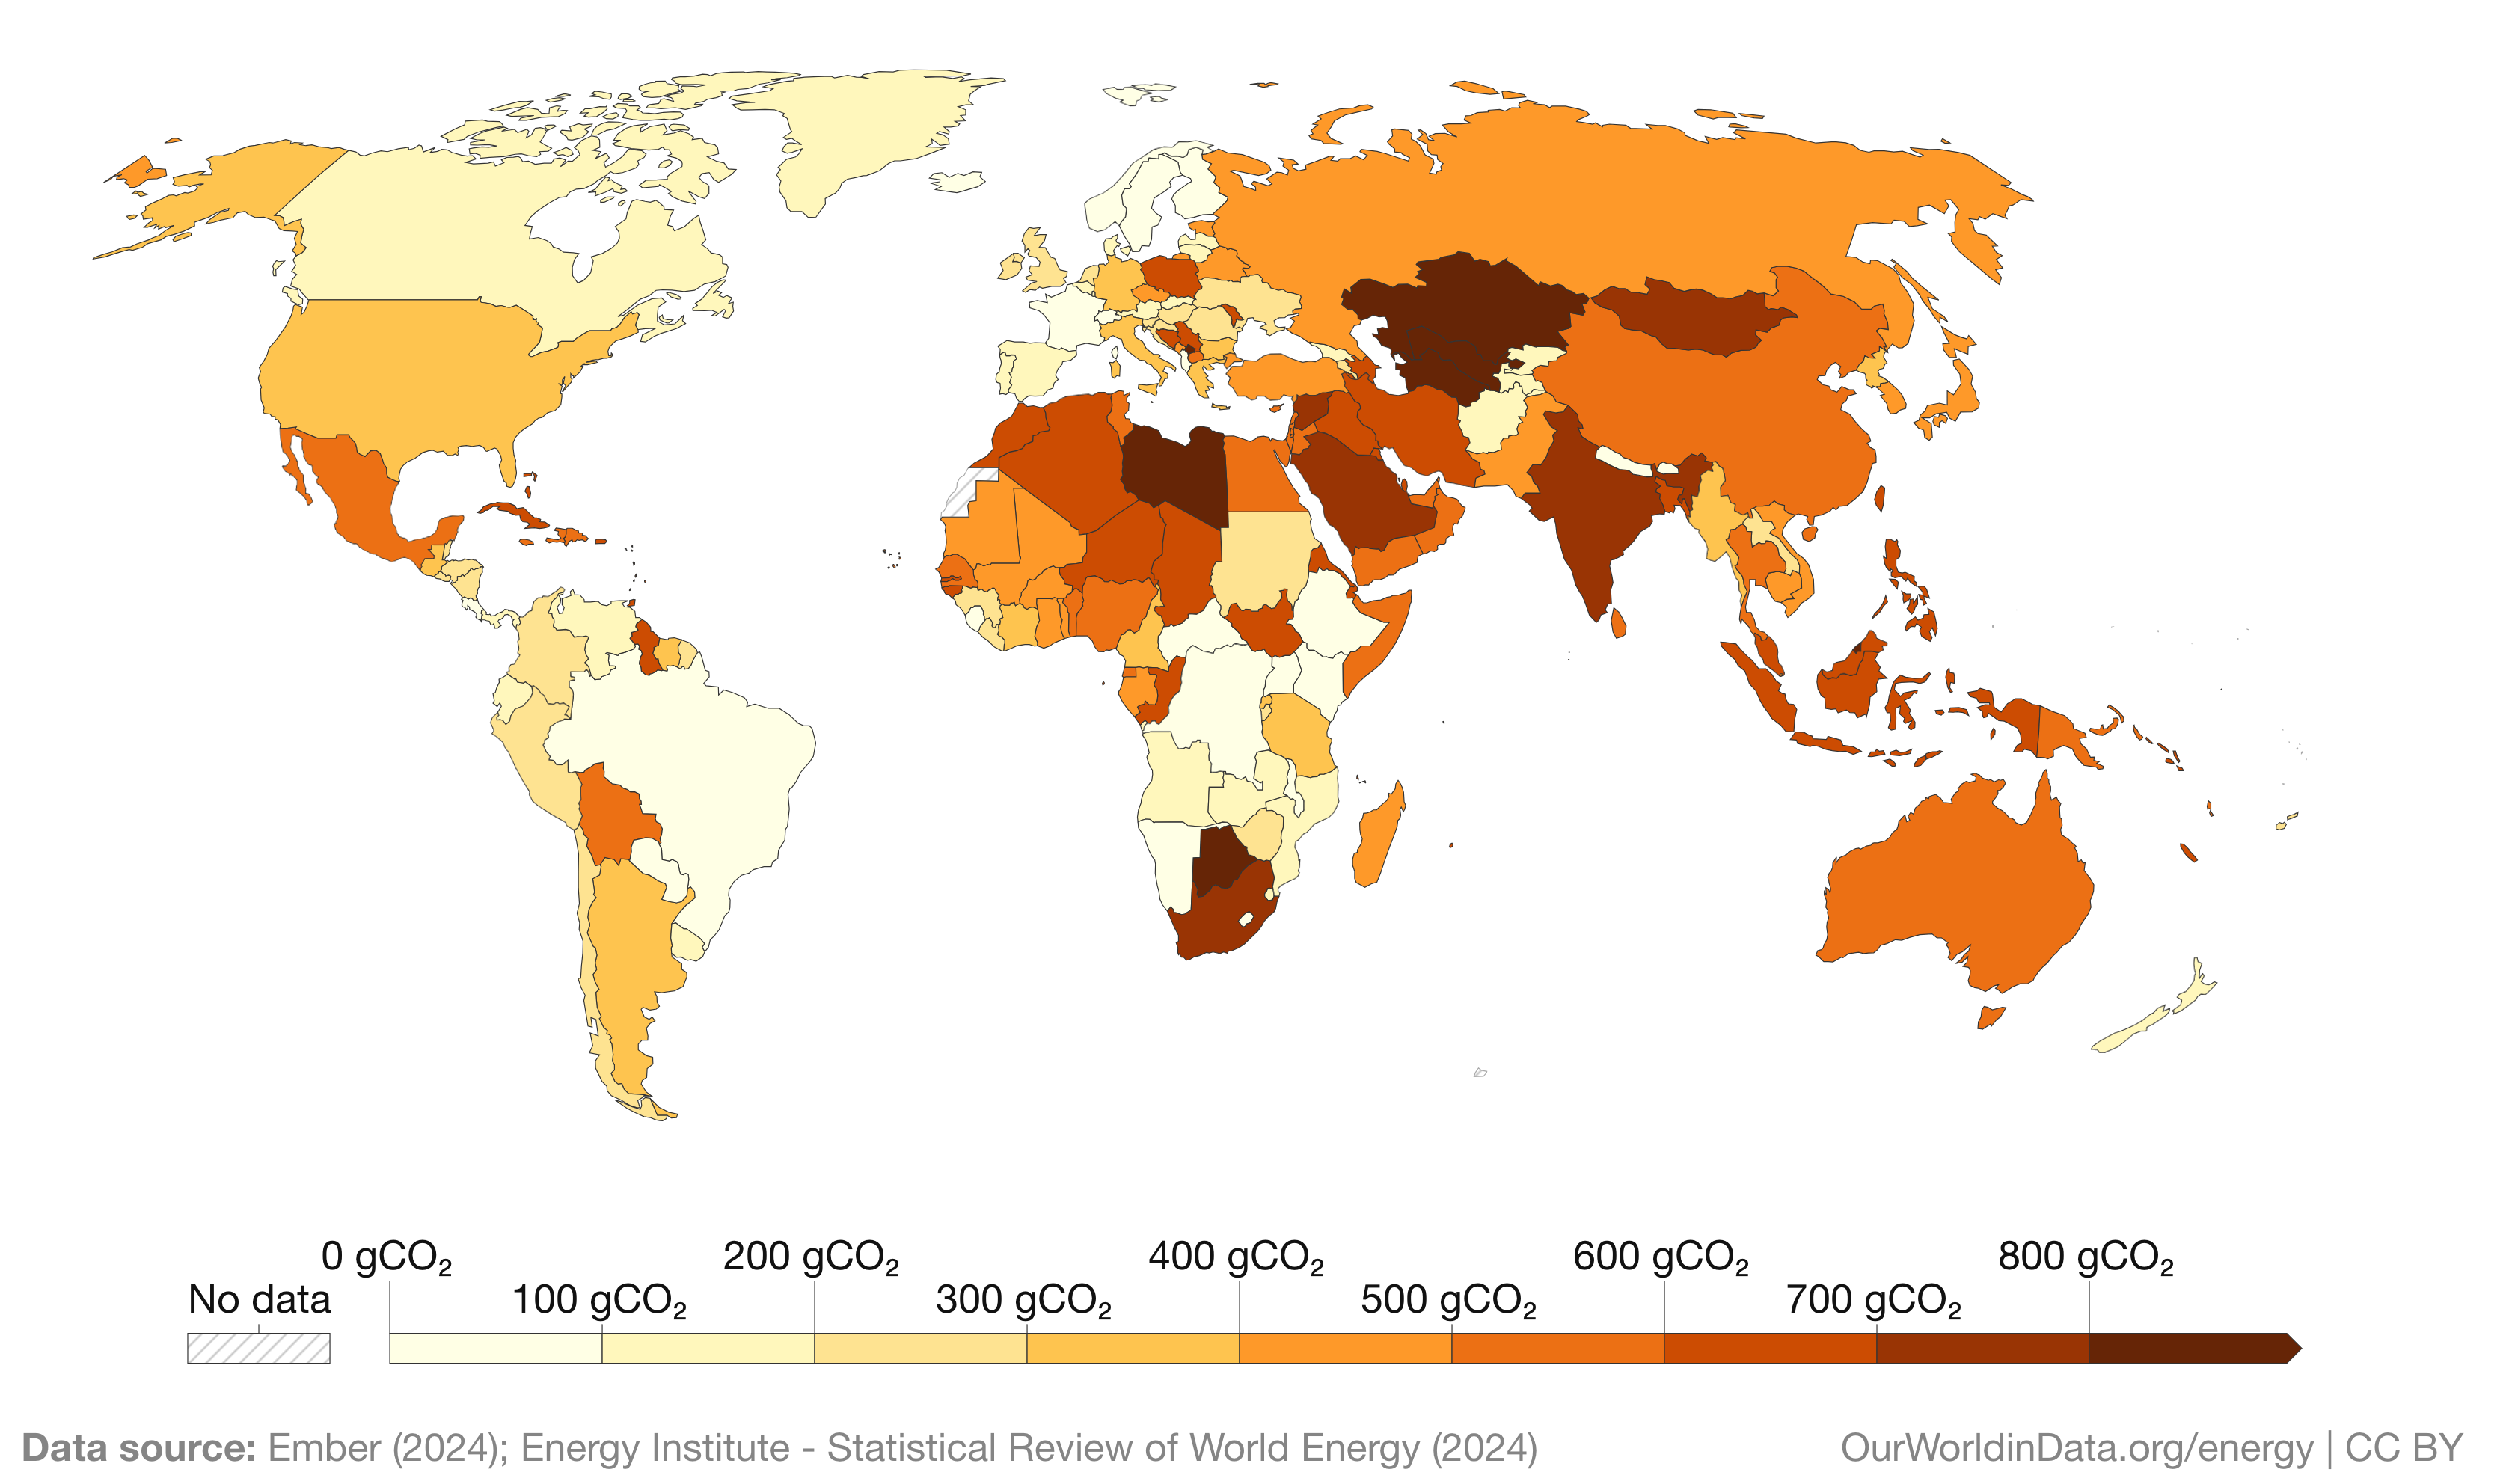
\includegraphics[width=\linewidth]{imgs/carbon-intensity-electricity.png}
    \caption{Carbon intensity of electricity generation, 2023. Source \cite{ember2024carbonintensity}}
    \label{fig:carbon_intensity}
\end{figure}

\section{Extending HADA with CodeCarbon}

\subsection{Energy Management Algorithms}

The first step to extend HADA with Carfon Intensity is therefore to gather a dataset which includes data about carbon footprint 
of the algorithms execution, integrating CodeCarbon in code for running our algorithms. The first two algorithms that were analysed 
are ANTICIPATE and CONTINGENCY, introduced in \cite{ijcai2019p150} \cite{10.1007/978-3-319-93031-2_8} and used in the HADA paper to present the framework \cite{DEFILIPPO2022109199}.
These are two Stochastic Algorithms from the energy management system domain, which calculate the amount of energy that must be 
produced by the energy system to meet the required load, minimising the total energy cost over the daily time horizon and by taking 
into account the uncertainty. In particular, ANTICIPATE is an online (scenario-based) anticipatory algorithm, while CONTINGENCY 
is an integrated offline/online algorithm that tackles the uncertainty by building (offline) a pool of solutions to guide an 
efficient online method. Both these methods are characterized by a parameter that can be changed based on the required constraints
in terms of time constraint and required solution quality (resp., the number of scenarios for ANTICIPATE, and the number of traces 
for CONTINGENCY). The goal of HADA is to learn the relationship between this configuration parameter and a series of performance
metrics which describes the Resource Usage of the Algorithm and the quality of the solution. The dataset used originally in HADA then
includes the following attributes:

\begin{itemize}
    \item \verb|nParam|: Value of the algorithm configuration parameter, i.e. \verb|nScenarios| For ANTICIPATE and \verb|nTraces| for CONTINGENCY;
    \item \verb|time(s)|: Time required to find a solution;
    \item \verb|sol(keuro)|: Cost of the solution found (expresses solution quality);
    \item \verb|memAvg(MB)|: Average memory used by the algorithm.
\end{itemize}

As already mentioned, we would like to extend this work by considering also the algorithm performance in terms of Energy Consumption and
Carbon Footprint. We then added the following metrics taken from CodeCarbon:

\begin{itemize}
    \item \verb|emissions|: the total emissions of $\mathsf{CO_2e}$ (kg)
    \item \verb|emission_rate|: the amount of $\mathsf{CO_2e}$ emissions per second (kg/s);
    \item \verb|cpu_energy|: the energy consumed by the cpu;
    \item \verb|ram_energy|: the energy consumed by the ram;
    \item \verb|tot_energy|: the total energy consumed;
    \item \verb|country| and \verb|region|: the country and region where the computation took place;
    \item \verb|cpu_count|: the number of cores.
\end{itemize}

In addition to these, we also implemented the tracking of the peak memory usage (which we called \verb|memPeak(MB)| in the dataset).

\subsection{Min-Cut/Max-Flow Algorithms}

After ANTICIPATE and CONTINGENCY, that were already included in HADA, we decided that it would be interesting to further extend HADA
with new algorithms. We opted for a set of algorithms used to solve Minimum Cut/Maximum Flow problems on Graphs, that are used for a4paper
number of Computer Vision tasks. We reffered to the work of Jensen et al. (2023) \cite{Jensen2023Maxflow}, that offers a review of 
Min-Cut/Max-Flow state-of-the-art algorithms, evaluated on a large Dataset of Computer Vision problems. In particular, we focused on
three algorithms:

\begin{itemize}
\item Boykov-Kolmogorov (BK)
\item Excess Incremental Breadth First Search (EIBFS)
\item Hochbaum's Pseudo Flow (HPF)
\end{itemize}

Accoring to Jensen et al. there are different families of Min-Cut/Max-Flow algorithms. BK belongs to the so called Augmenting Paths (AP)
family, which is the oldest one, introduced with the Ford-Fulkerson Algorithm [insert citation]. Instead, EIBFS and HPF are from the family of the so 
called \textit{Pseudoflow} algorithms [insert citation]. The main differences are the order in which they scan through nodes when looking for an arc 
connecting two trees in the forest, and how they push flow along the paths.

Differently from ANTICIPATE and CONTINGENCY, these algorithms does not have a configuration parameter. Since these three algorithms can 
be implemented in different variants, we decided to treat the algorithm's implementation type as a configuration parameter. The variants considered
are the following:

\begin{itemize}
    \item For Boykov-Kolmogorov we considered:
    \begin{itemize}
        \item The reference implementation (BK);
        \item The implementation by Jensen et al. (MBK), with several optimisations, such as using indices instead of pointers to reduce memory footprint;
        \item A second implementation by Jensen et al. (MBK-R) which reorders arcs, so that all outgoing arcs from a node are adjacent in memory.
    \end{itemize}
    \item For Excess Incremental Breadth First Search we considered:
    \begin{itemize}
        \item A slightly modified version of original algorithm (EIBFS);
        \item A second version replacing pointers with indices (EIBFS-I);
        \item A third version without arc reordering (EIBFS-I-NR).
    \end{itemize}
    \item For Hochbaum's Pseudo Flow we considered:
    \begin{itemize}
        \item Highest label variant, with FIFO buckets (HPF-H-F);
        \item Highest label variant, with LIFO buckets (HPF-H-L);
        \item Lowest label variant, with FIFO buckets (HPF-L-F);
        \item Lowest label variant, with LIFO buckets (HPF-L-L).
    \end{itemize}
\end{itemize}

Jensen et al. provided a series of scripts to evaluate the runtime of those algorithms - considering both the initialization time and the time required
to come up with a solution. In order to monitor our target metrics, we wrapped the algorithms scripts - which are implemented in C++ code - with a Python
script that implements memory usage tracking and uses CodeCarbon to monitor Energy Usage and Carbon Emissions. Differently from ANTICIPATE and CONTINGENCY
here we do not take the solution quality into consideration.

\chapter{Experimental Analysis}

\section{Benchmarking on Different Hardware Platforms}

For the benchmark phase, we opted for running the algorithms on different Hardware Platforms, in order to better capture the differences in performance
when changing the machine on which the algorithm is executed:

Experiments were conducted on:
\begin{itemize}
\item \verb|mbp19|: A Laptopr running MacOS Ventura 13.6.7 with:
    \begin{itemize}
        \item 1,4 GHz Quad-Core Intel Core i5;
        \item 8 GB 2133 MHz LPDDR3;
    \end{itemize}
\item \verb|PC|: A PC with Ubuntu 22.0.4 LTS
\item \verb|leonardo| An HPC infrastructure, i.e. Leonardo hosted by CINECA. It has a total of 4992 computing nodes organized in two partitions, the Booster partition and the Data Centric General Purpose (DCGP) partition. For running the benchmark phase we used the booster partition, which has the following specifics:
    \begin{itemize}
        \item 8×64 GB DDR4 3200 MHz (512 GB)
        \item single socket 32-core Intel Xeon Platinum 8358 CPU, 2.60GHz (Ice Lake) (110592 cores).
        \item 4x NVIDIA custom Ampere A100 GPU 64GB HBM2e, NVLink 3.0 (200GB/s)
    \end{itemize}
\end{itemize}

ANTICIPATE and CONTINGENCY were executed on 30 instances which were sampled with a statistical model with a Gaussian distribution \cite{DEFILIPPO2022109199}.
On each instance, each algorithm was executed with parameter (i.e. number of traces or scenarios) values ranging from 1 to 100. For ANTICIPATE and CONTINGENCY we
used only \verb|mbp19| and \verb|leonardo|. Thus in the end we obtained a dataset with a total of $30 \times 100 \times 2 \times 2 = 12,000$ entries. 

To generate a benchmark dataset for the Min-Cut/Max-Flow algorithms, we relied on the dataset provided by [Insert source]. This is an extensive collection of instances
of Min-Cut/Max-Flow problems in the Computer Vision field. The authors also provided the implementations of the algorithms that were used to generate our benchmark data.
Since they are implemented in C++ (BK and EIBFS) and C (HPF), we faced the problem of how to track the energy consumption and thus the emissions of such code. Apparently,
there are not much tool available to monitor the emissions of C code. % TODO: expand this in the RELATED WORK SECTION.
We opted for using a python wrapper script, that runs the C++/C scripts implementing the algorithms and uses CodeCarbon to track the energy consumption of the script execution.
For reasons due to lacking support on MacOS, i was not able to compile the BK and EIBFS implementation on mbp19. Instead, i have managed to restore an old PC i had at home 
with a light distribution of Ubuntu to run some of these scripts. 
It is important to point out that we did not executed the selected algorithms on the whole dataset, since some of the problem instances were very big, sometimes exceeding the available memory,
we just ran a subset of them - even if it was possible to create a swap partition big enough to accomodate bigger instances, the monitoring tools available just record the 
used RAM, so the estimate of the memory usage would be downsized in such cases. Also, due to the large number of instances, running a benchmark phase on all of them would have
been way too time consuming. 

\subsection{ANTICIPATE and CONTINGENCY}

% BOX PLOTS

\begin{figure}[h!]
    \centering
    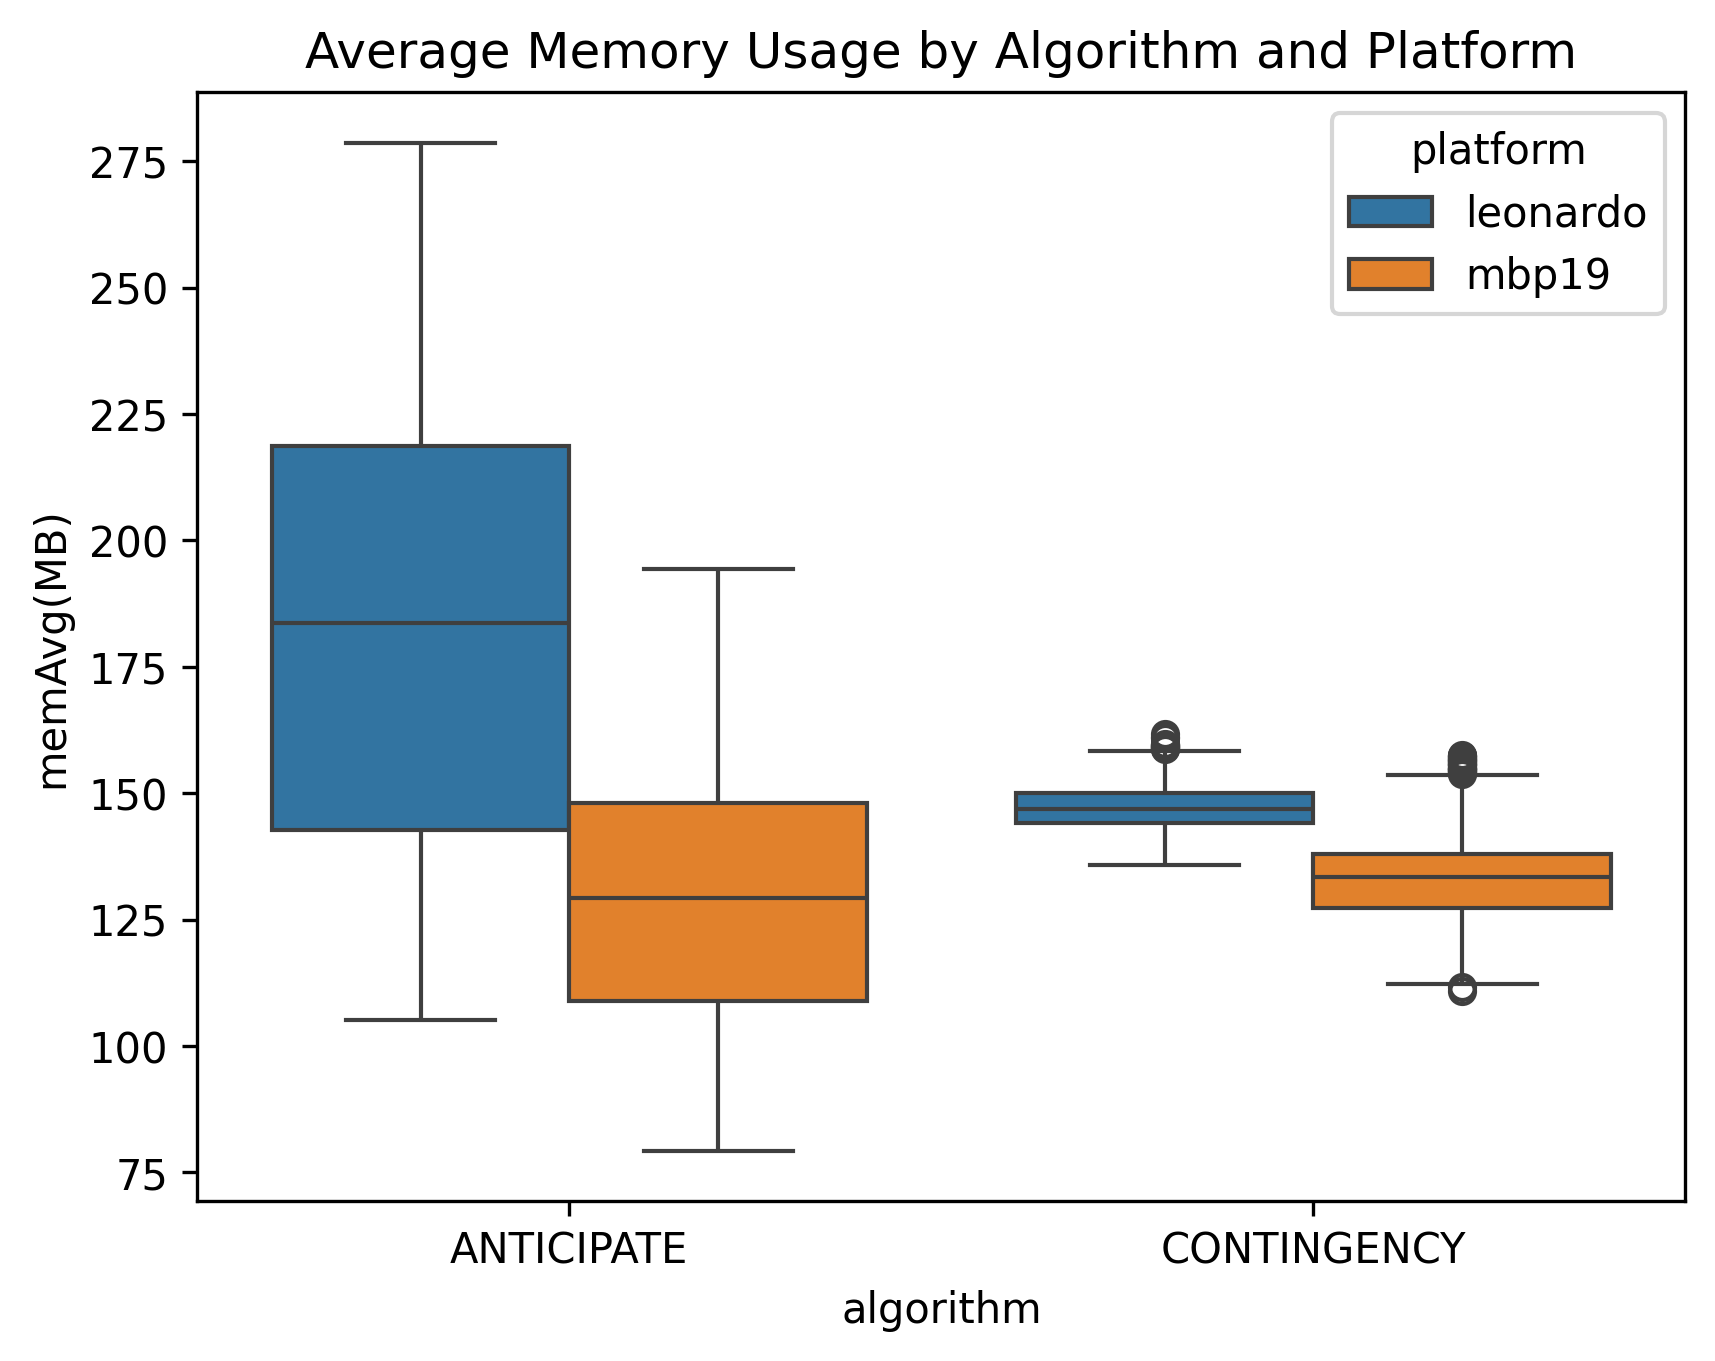
\includegraphics[width=0.8\textwidth]{imgs/avg_mem_usage.png}
    \caption{Average memory usage of ANTICIPATE and CONTINGENCY divided by platform}
    \label{fig:ant_cont_avg_mem_usage}
\end{figure}

\begin{figure}[h!]
    \centering
    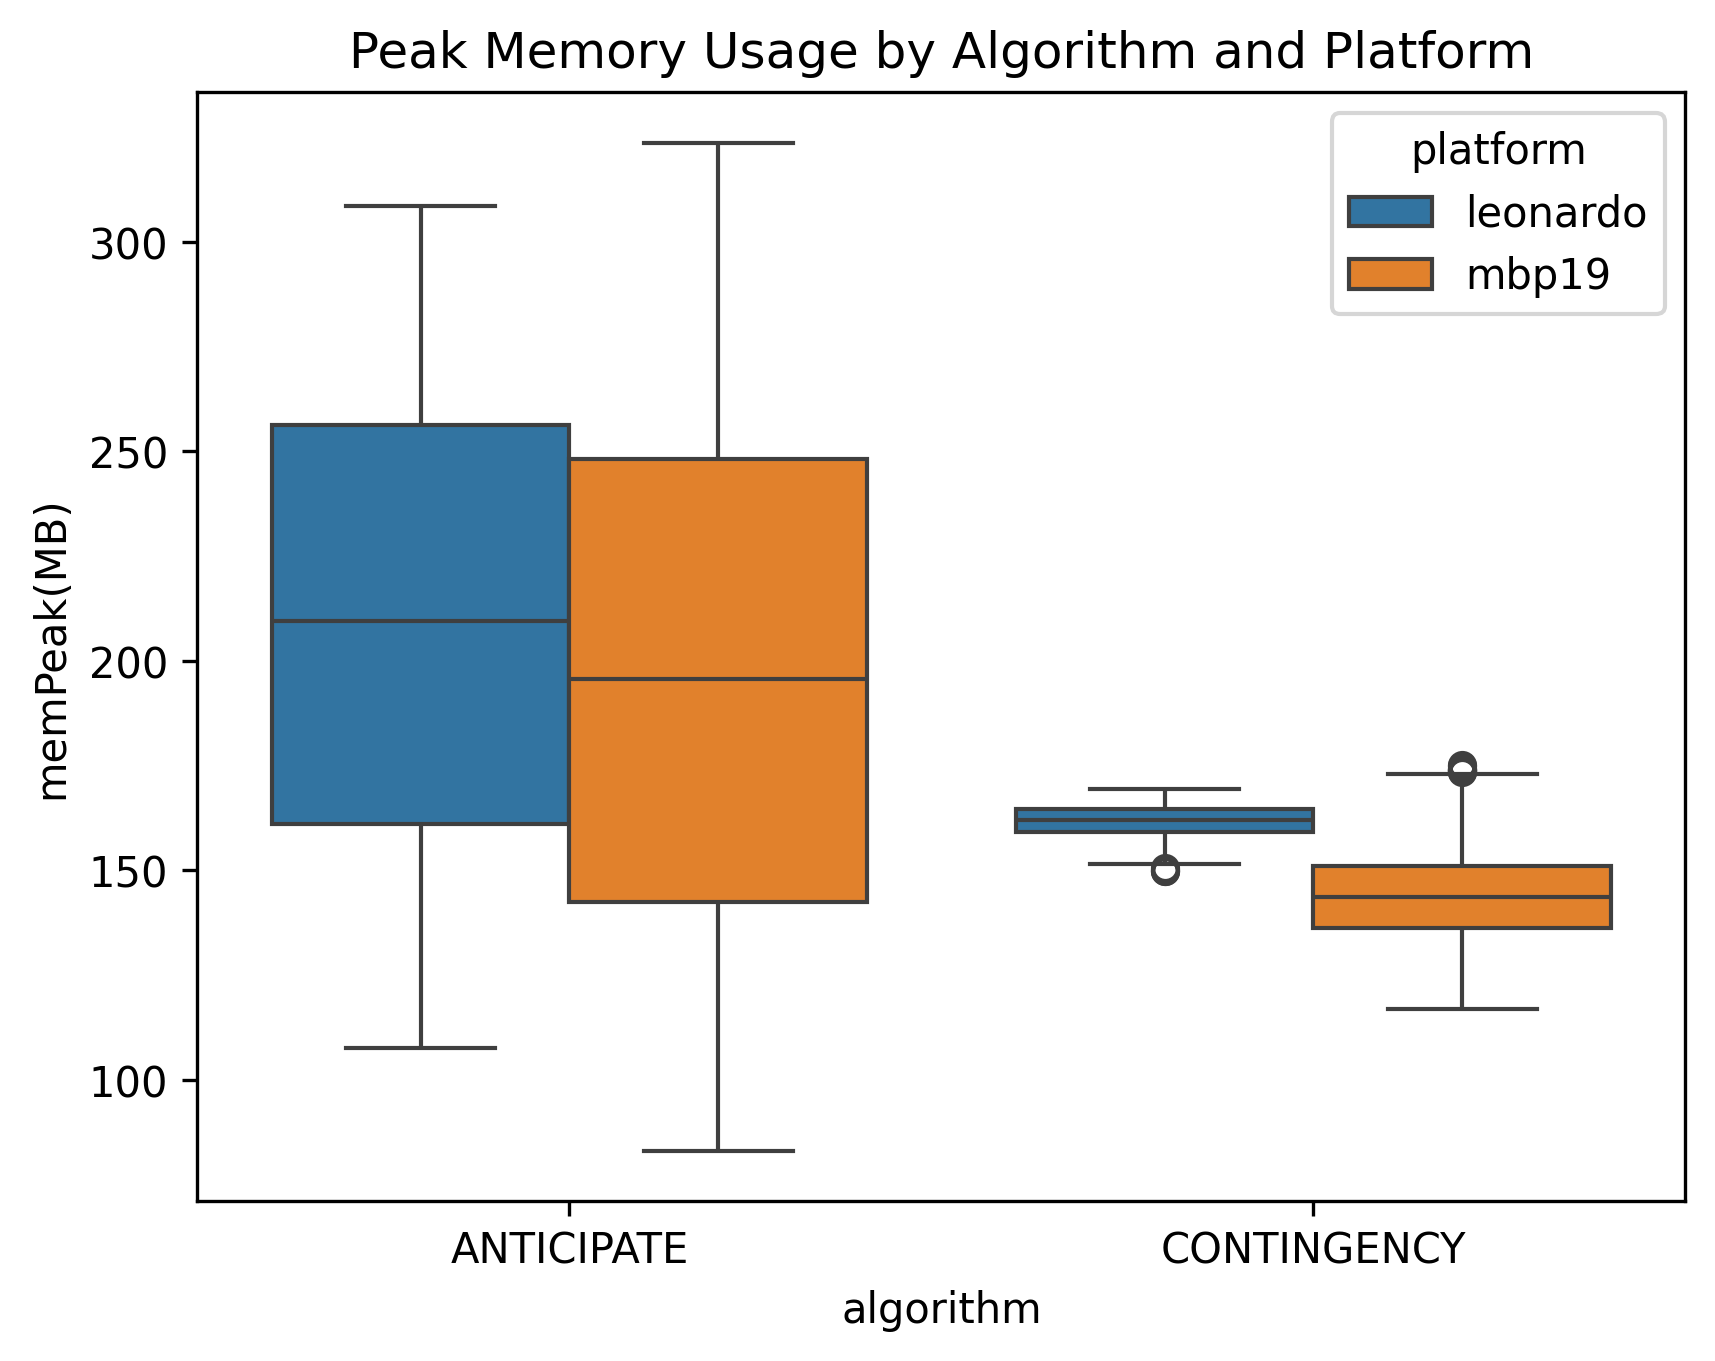
\includegraphics[width=0.8\textwidth]{imgs/peak_mem_usage.png}
    \caption{Peak memory usage of ANTICIPATE and CONTINGENCY divided by platform}
    \label{fig:ant_cont_peak_mem_usage}
\end{figure}

\begin{figure}[h!]
    \centering
    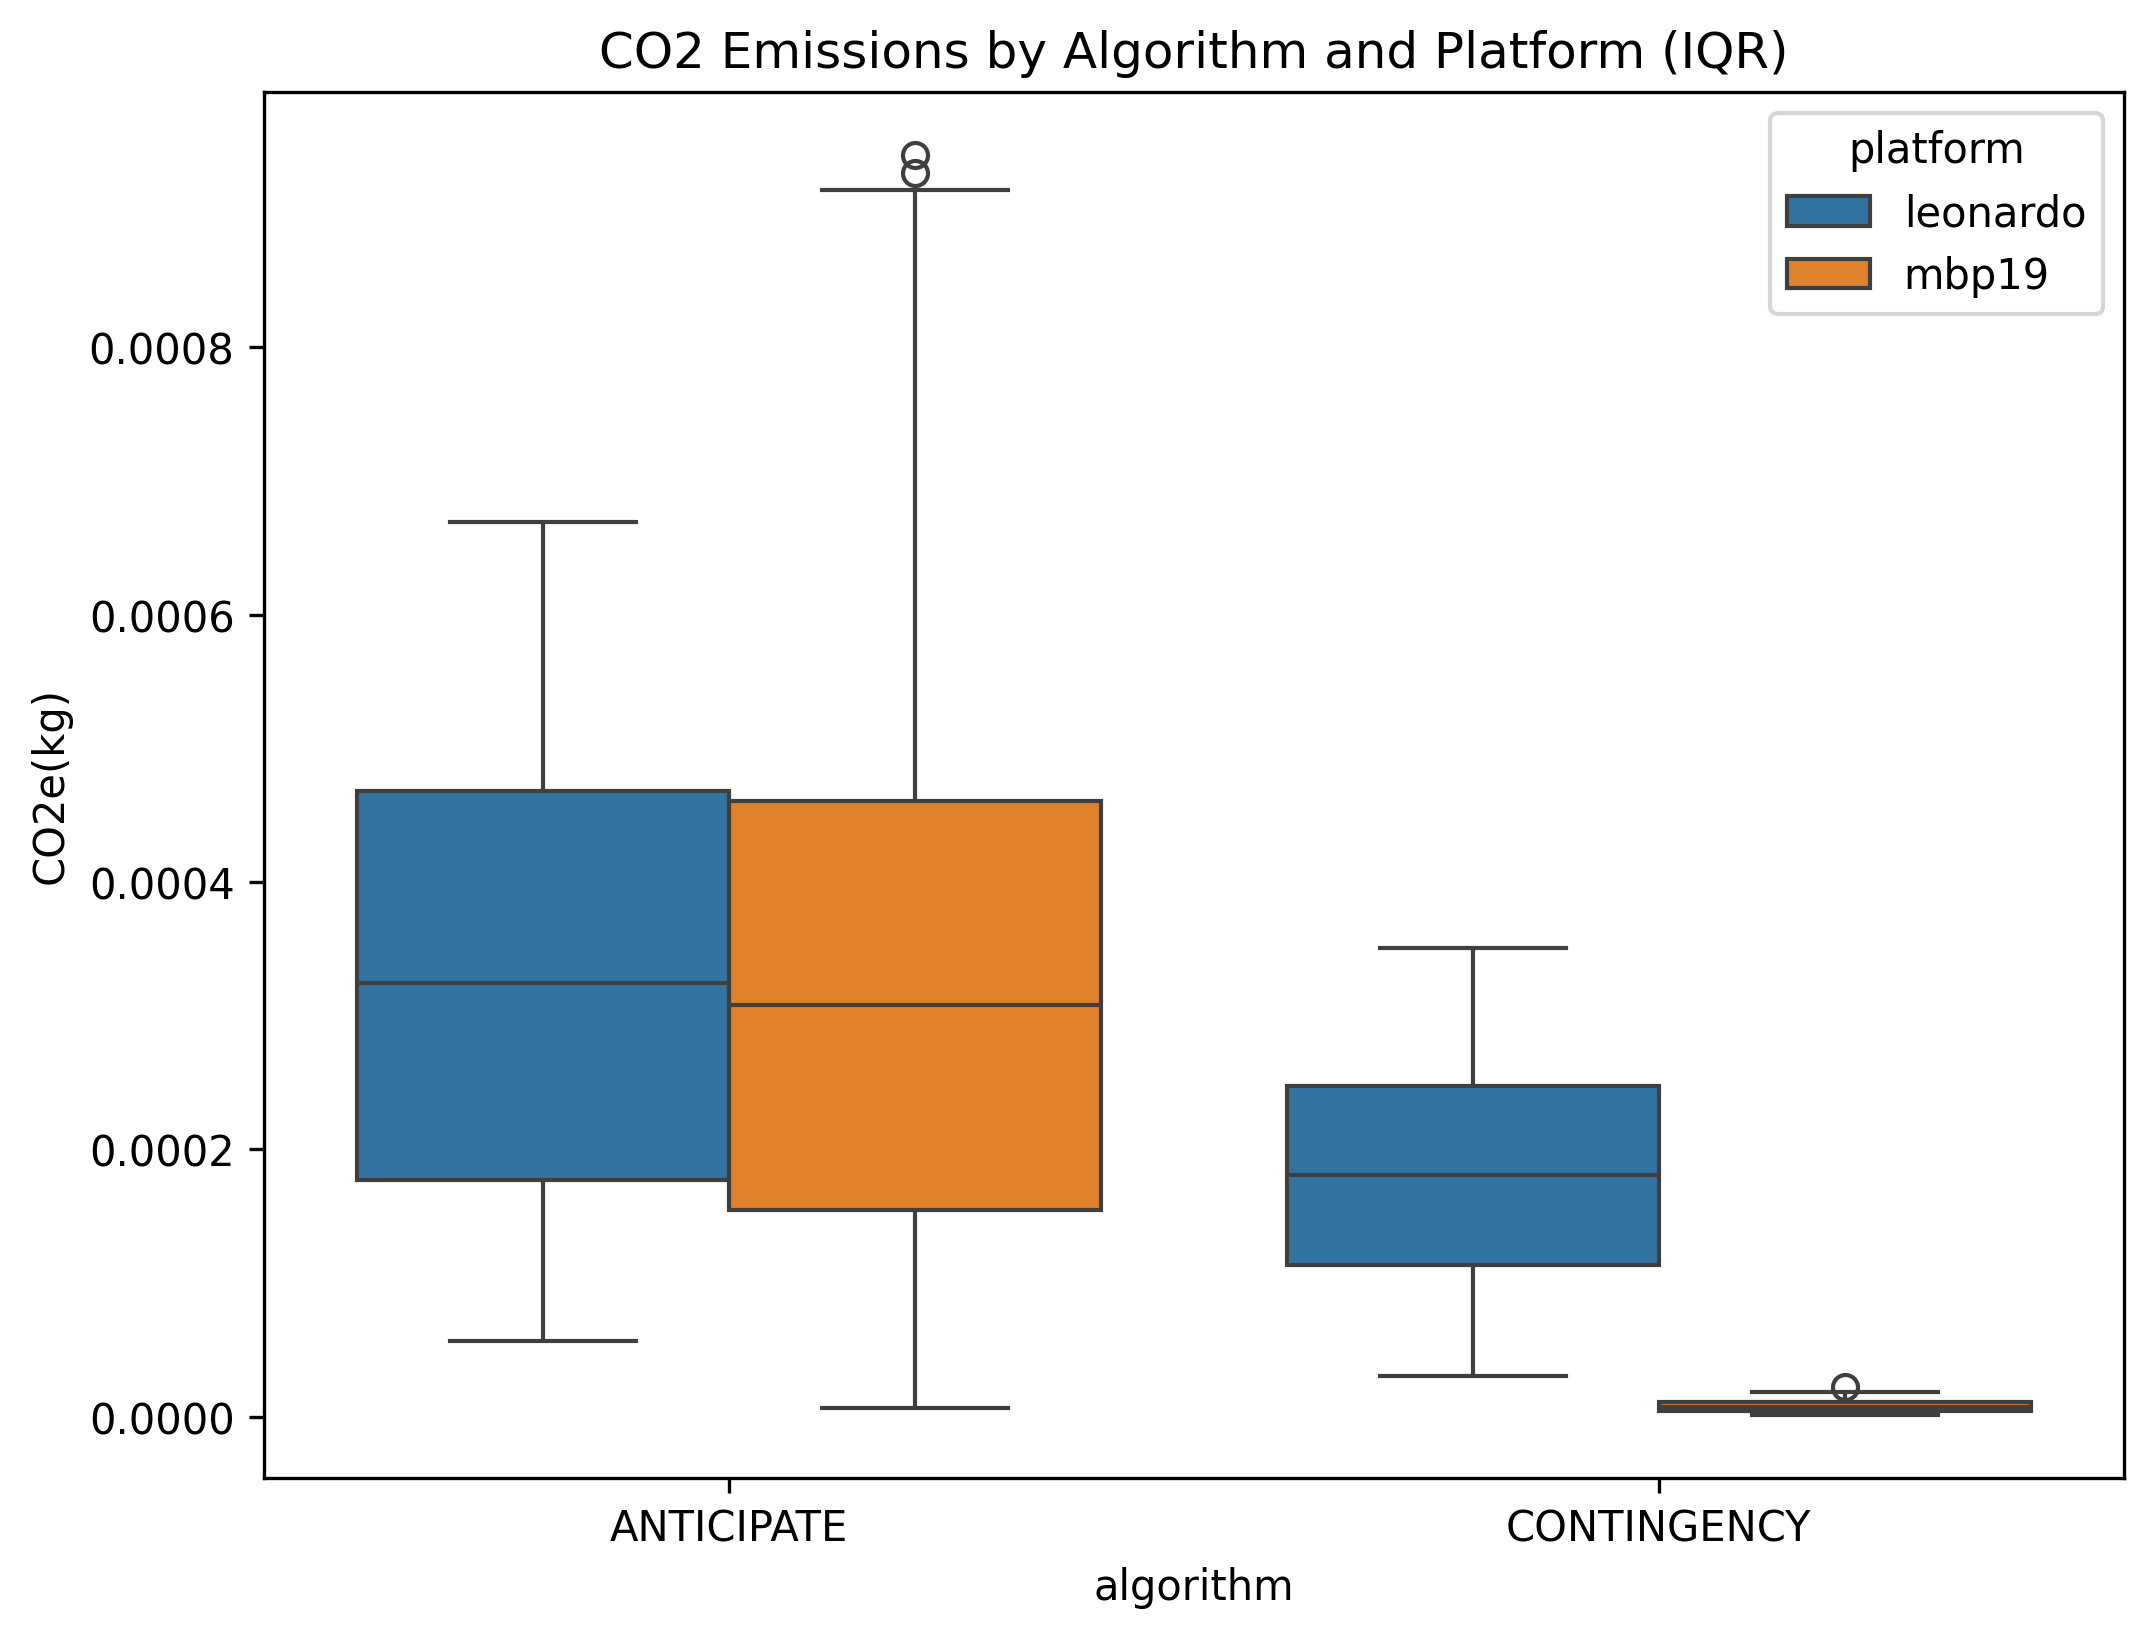
\includegraphics[width=0.8\textwidth]{imgs/CO2_emissions_no_outliers.png}
    \caption{CO2 emissions for ANTICIPATE and CONGINGENCY ordered by platform}
    \label{fig:ant_cont_co2_emissions}
\end{figure}

\begin{figure}[h!]
    \centering
    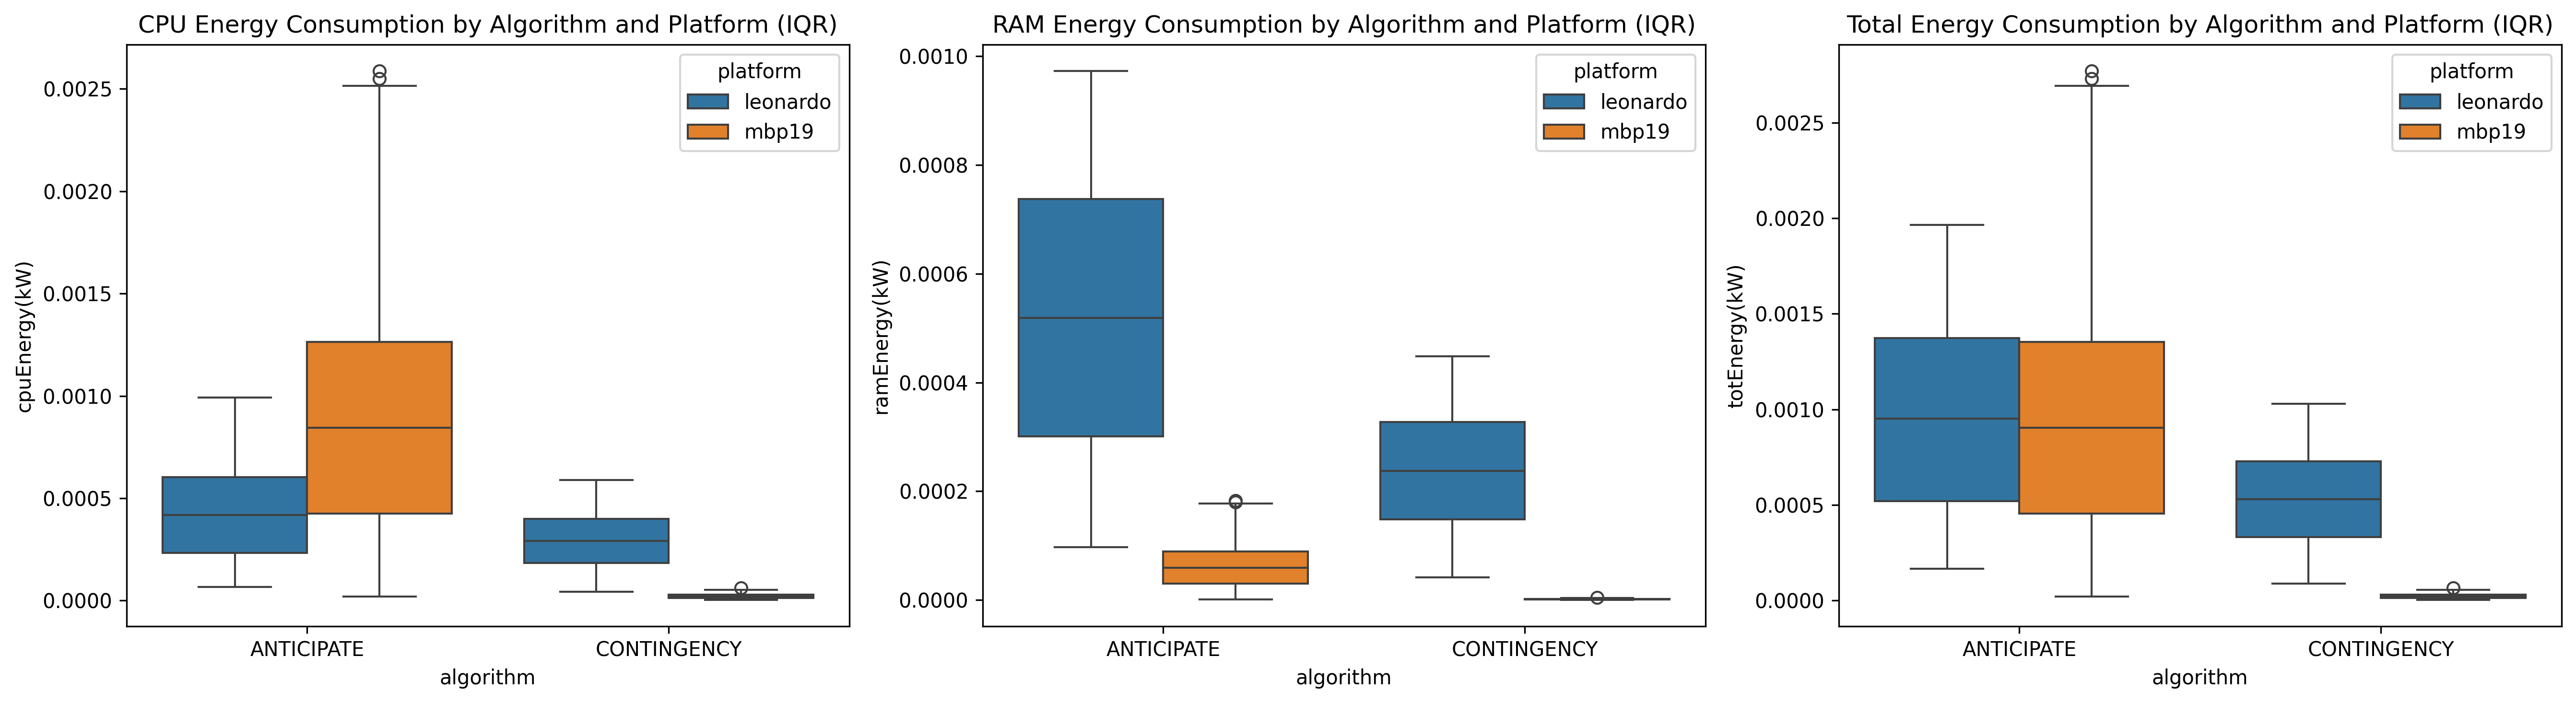
\includegraphics[width=0.8\textwidth]{imgs/energy_consumption_no_outliers.png}
    \caption{Energy Consumption data for ANTICIPATE and CONTINGENCY}
    \label{fig:ant_cont_energy}
\end{figure}

% CORRELATION MATRICES

\begin{figure}[h!]
    \centering
    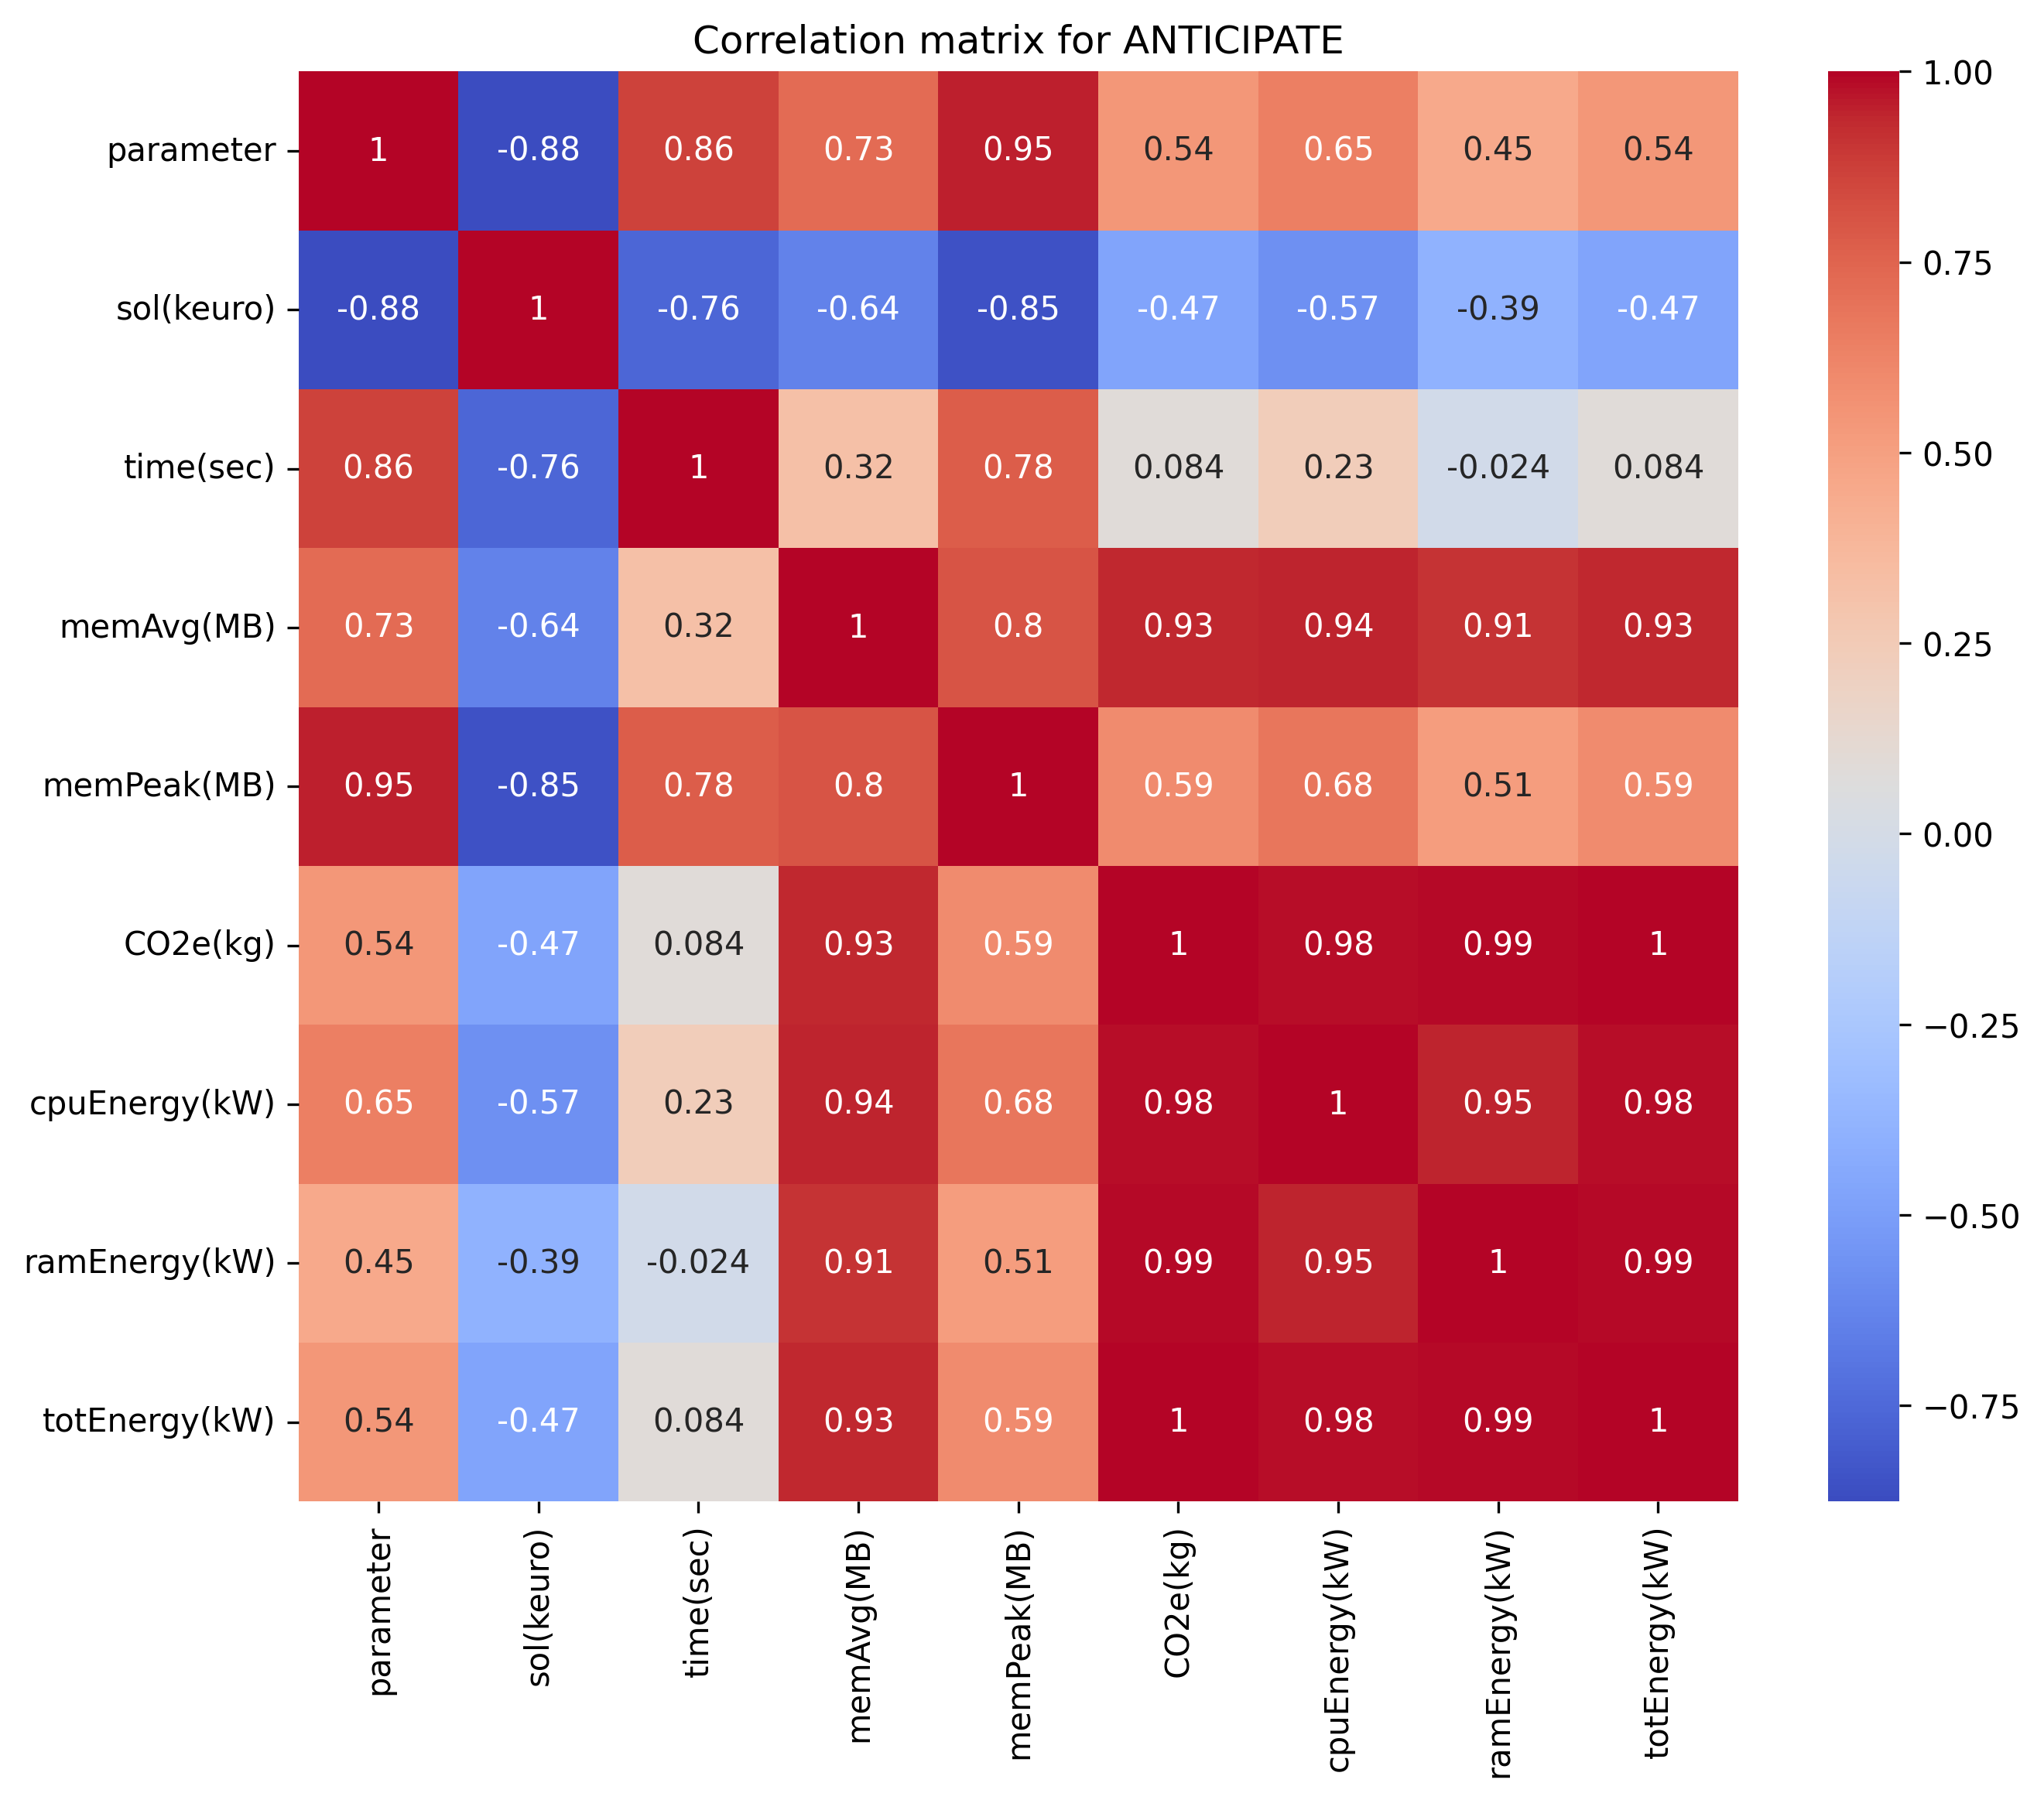
\includegraphics[width=0.8\textwidth]{imgs/ant_corr_mat.png}
    \caption{Correlation matrix for ANTICIPATE}
    \label{fig:ant_corr_mat}
\end{figure}

\begin{figure}[h!]
    \centering
    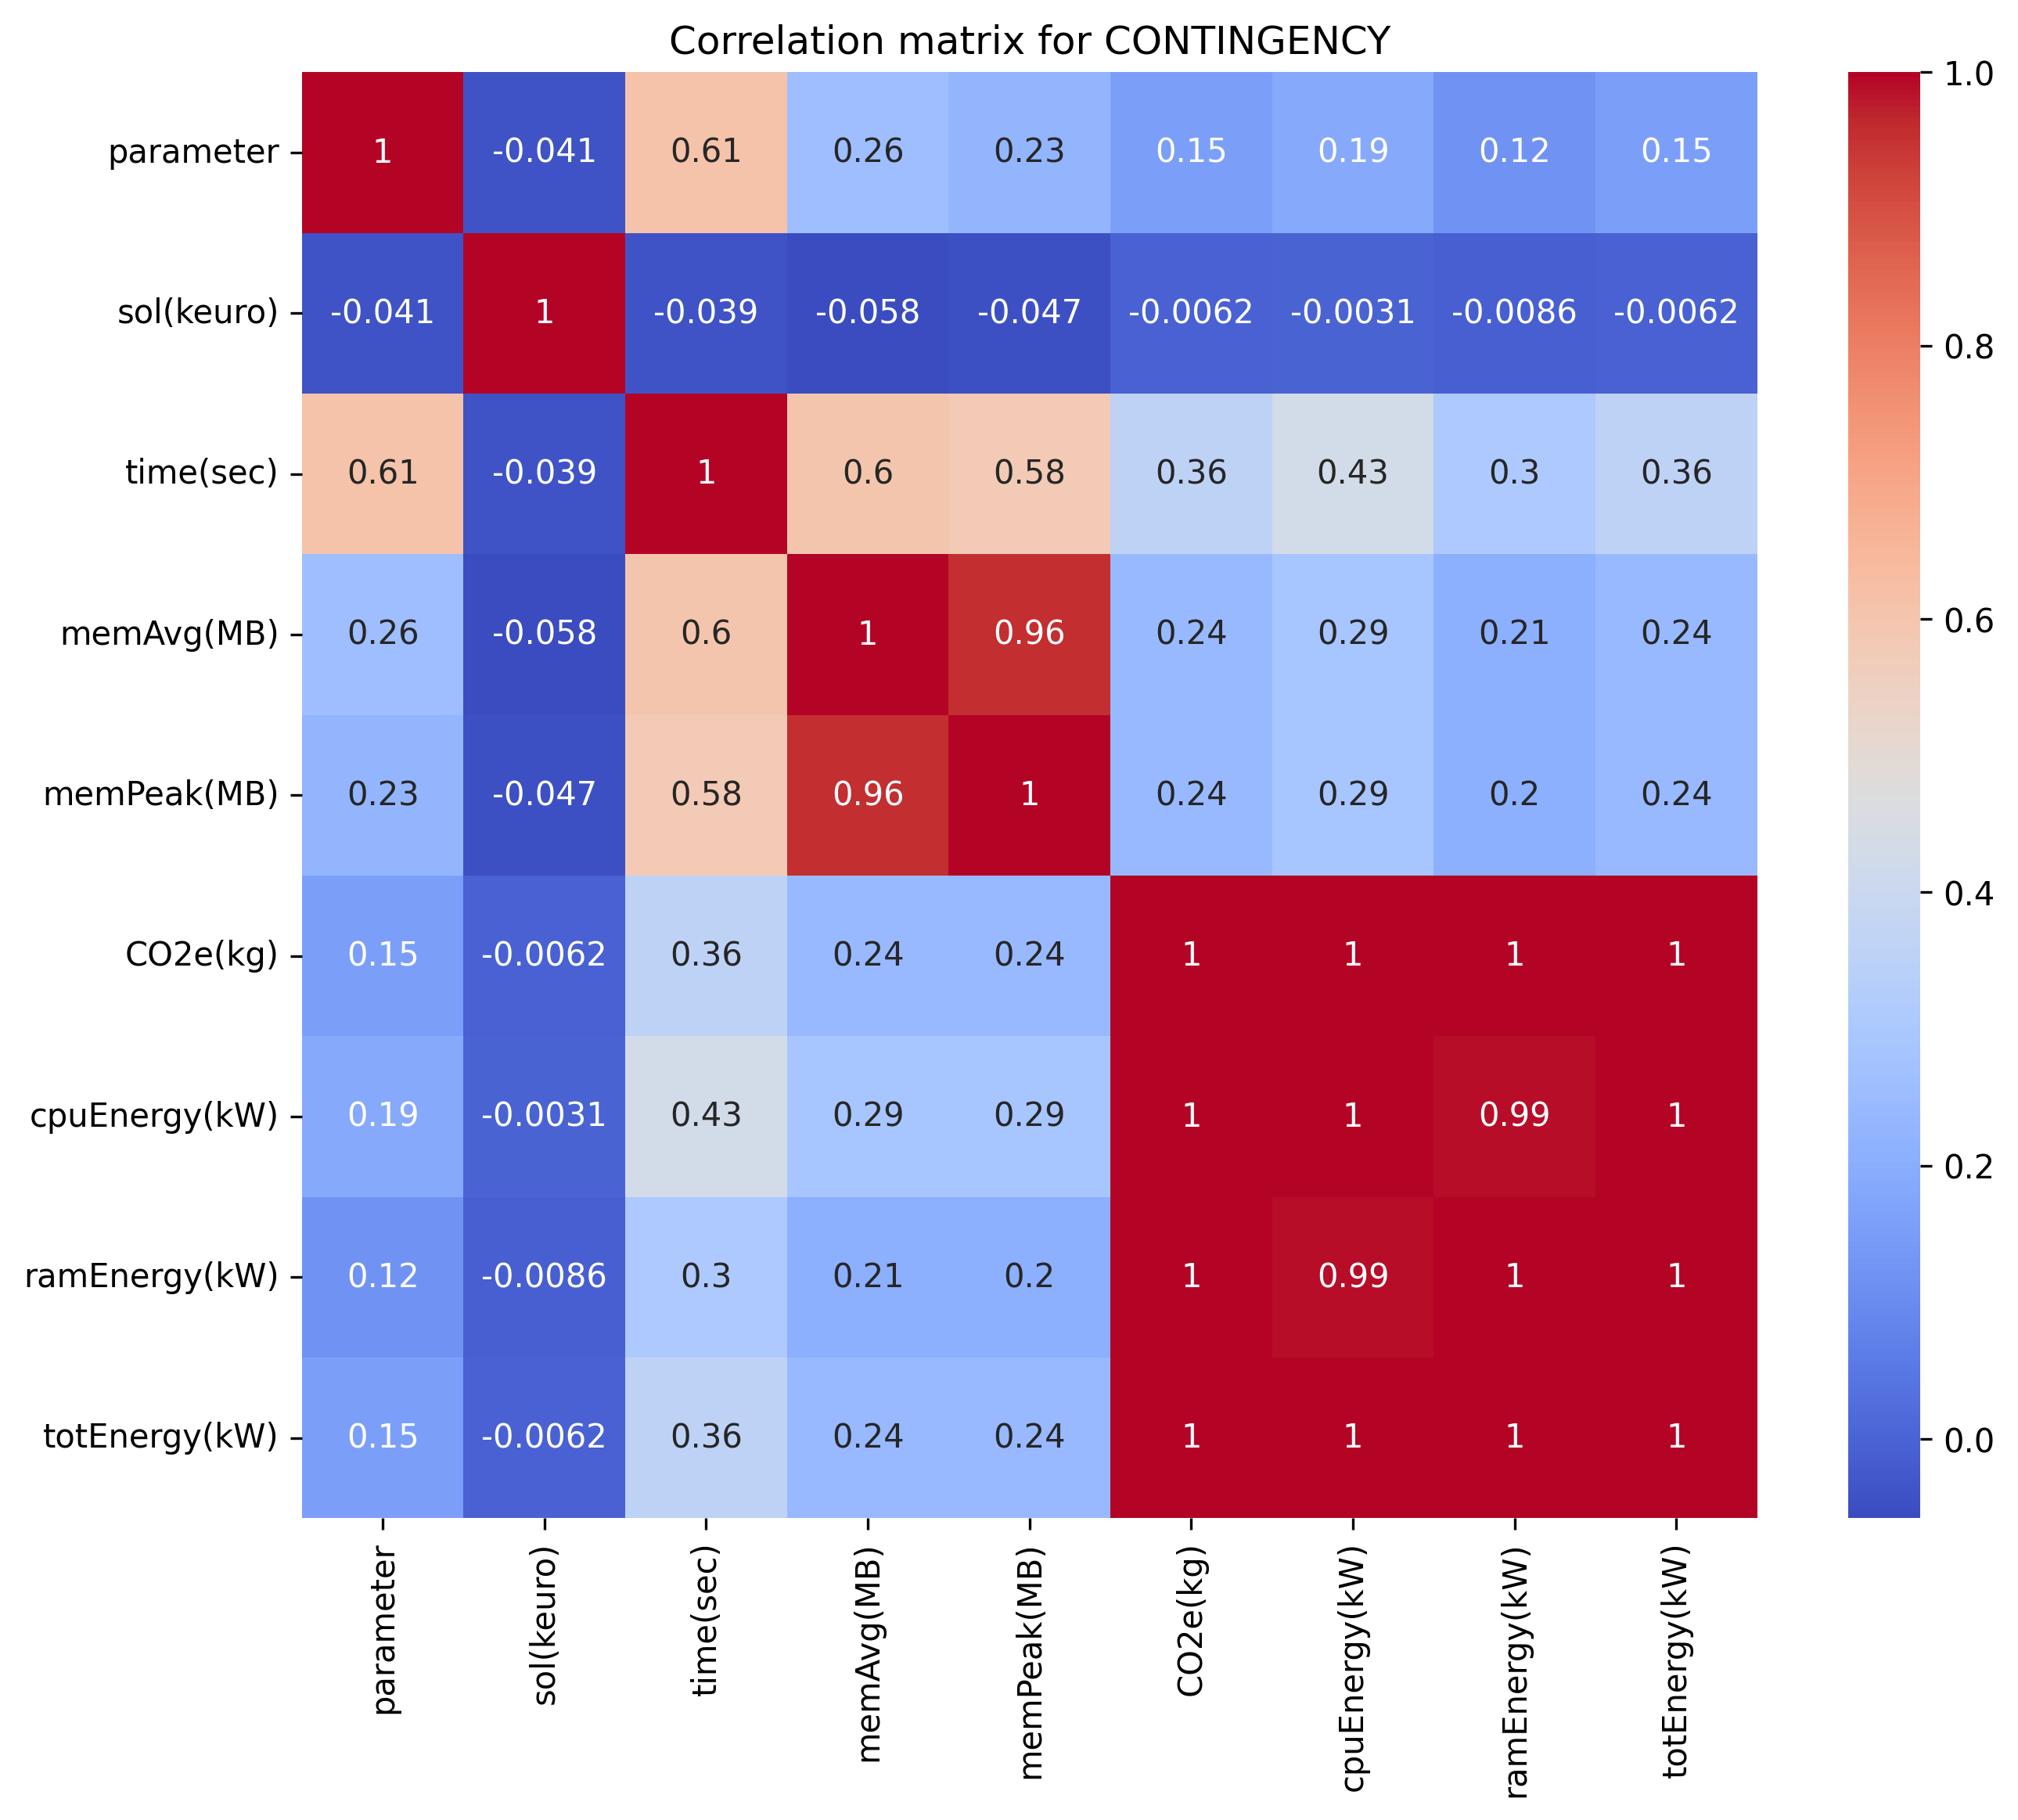
\includegraphics[width=0.8\textwidth]{imgs/cont_corr_mat.png}
    \caption{Correlation matrix for CONTINGENCY}
    \label{fig:cont_corr_mat}
\end{figure}

Here we can see some results given by the HADA framework tested on the updated dataset for ANTICIPATE and CONTINGENCY. \ref{tab:anticipate_results}
presents the results of optimising any target without any constraints for ANTICIPATE. We can notice how, for most metrics keeping the number of scenarios
as low as possible is the best choice, while increasing them brings the solution cost down.

\begin{table}[h!]
    \centering
    \begin{tabular}{|c|ccc|}
        \hline
        \multicolumn{1}{|c|}{Objective} & \multicolumn{3}{c|}{Solution} \\
        \hline
        Target & $n^P$ & HW & Value \\
        \hline
        CO2e (kg) & 1 & mbp19 & $7.23 \times 10^{-6}$ \\
        Cost (€) & 97 & mbp19 & $267.39k$ \\
        Time (s)& 1 & mbp19 & $1.24$ \\
        Avg. Memory (MB) & 1 & mbp19 & $81.47$ \\
        Peak Memory (MB) & 2 & mpb19 & $92.19$ \\
        Energy (kW) & 1 & mbp19 & $2.12$ \\
        \hline
    \end{tabular}
    \caption{Minimum values for each target for the ANTICIPATE algorithm}
    \label{tab:anticipate_min_targets}
\end{table}

% TODO: check minimum values of other metrics too

\begin{table}[h!]
    \centering
    \begin{tabular}{|c|ccc|}
        \hline
        \multicolumn{1}{|c|}{Objective} & \multicolumn{3}{c|}{Solution} \\
        \hline
        Target & $n^P$ & HW & Value \\
        \hline
        CO2e (kg) & 2 & mbp19 & $1.28 \times 10^{6}$ \\
        Cost (€) & 90 & mbp19 & $314.11k$ \\
        Time (s)& 1 & mbp19 & $5.16$ \\
        Avg. Memory (MB) & 1 & mbp19 & $117.66$ \\
        Peak Memory (MB) & 2 & mbp19 & $130.58$ \\
        Energy (kW) & 2 & mbp19 & $3.77 \times 10^{-6}$ \\
        \hline
    \end{tabular}
    \caption{Minimum values for each target for the CONTINGENCY algorithm}
    \label{tab:contingency_min_targets}
\end{table}

As we can see in \ref{fig:ant_corr_mat}, \verb|totEnergy| has a correlation of $1$ with CO2e, meaning they are perfectly proportional to each other. This reflects the fact that Carbon Emissions,
as measured by CodeCarbon, depends by two factors, i.e. the energy consumed by running the algorithm and the Carbon Intensity. Since we executed all the experiments in the same
country, the Carbon Intensity over the whole dataset is fixed, meaning that the only factor influencing the CO2e emissions is the energy consumed, while the Carbon Intensity
is just a scaling factor. Indeed, \verb|totEnergy| and \verb|CO2e| both the same correlation values with the other variables. Also, as we could expect, the correlation
of \verb|CO2e| with \verb|cpuEnergy| and \verb|ramEnergy| is also pretty high, being of $0.98$ and $0.99$ respectively, and that reflects the fact that actually the total energy consumption is
nothing but the sum of \verb|cpuEnergy| and \verb|ramEnergy|. Then, as one may point out, we could just remove the energy consumption values from the dataset, and just keep the emissions.
However, the energy consumption values can be scaled by different Carbon Intensity values, giving the possibility of evaluating the impact of changing the location of the computations, as we will see later on.
Then, we can see that the average memory consumption is the variable with the highest correlation with the carbon emissions except for energy consumption, with a value of $0.93$. Then, we can see
that for ANTICIPATE the emissions are also influenced a bit by the value of the parameter ($0.65$) and the Solution Cost ($-0.57$). We could then perform some tests on ANTICIPATE with HADA
to asses the impact of constraints on memory and solution quality.

\begin{table}[h!]
    \centering
    \begin{tabular}{|cc|ccccc|}
        \hline
        \multicolumn{2}{|c|}{Bounds} & \multicolumn{5}{c|}{Solution} \\
        \hline
        Memory & Cost & $n^P$ & HW & CO2e & Memory & Cost \\
        \hline
        no & no & 1 & mbp19 & $7.23 \times 10^{-6}$ & - & - \\
        80 & no & none & none & none & none & none \\
        no & $100k$ & none & none & none & none & none \\
        100 & $300k$ & none & none & none & none & none \\
        150 & $300k$ & 64 & mbp19 & $3.75 \times 10^{-4}$ & $141.53$ & $299.46k$ \\
        170 & $270k$ & 97 & mbp19 & $5.70 \times 10^{-4}$ & $169.85$ & $267.39k$ \\
        170 & $280k$ & 87 & mbp19 & $5.10 \times 10^{-4}$ & $160.12$ & $276.86k$ \\
        300 & $500k$ & 1 & mbp19 & $7.23 \times 10^{-6}$ & $81.47$ & $368.73k$ \\
        \hline
    \end{tabular}
    \caption{Experimental results for the ANTICIPATE algorithm with bounds Memory usage and Solution cost}
    \label{tab:anticipate_results}
\end{table}

In \ref{tab:anticipate_results} we can see some the results of some combination of constraints on Solution cost (which is
expressed €), and Average Memory consumption (expressed in MB), with the objective of minimizing the CO2e 
emissions (in kg). The rows filled with "none" indicates that HADA didn't found a solution satisfying those constraints for the
given algorithm.

For CONTINGENCY, \ref{fig:cont_corr_mat} shows how the variables show very little amount of linear correlation between one another. The strongest relation is between the runtime and the amount of memory consumed
(with a score of $0.60$ for \verb|memAvg| and $0.58$ for \verb|memPeak|). As for the Carbon Footprint, the value that influence it the most is the runtime, with a postivie correlation of $0.47$.
So we will try to test HADA on CONTINGENCY with constraints on the Runtime (expressed in seconds), and the Solution cost.

\begin{table}[h!]
    \centering
    \begin{tabular}{|cc|ccccc|}
        \hline
        \multicolumn{2}{|c|}{Bounds} & \multicolumn{5}{c|}{Solution} \\
        \hline
        Time & Cost & $n^P$ & HW & CO2e & Time & Cost \\
        \hline
        no & no & 2 & mbp19 & $1.29 \times 10^{-6}$ & - & - \\
        no & $350k$ & 4 & mbp19 & $1.53 \times 10^{6}$ & - & $338.23k$ \\
        10 & no & 2 & mbp19 & $1.29 \times 10^{-6}$ & $6.01$ & - \\
        10 & $320k$ & none & none & none & none & none \\
        60 & $350k$ & 4 & mbp19 & $1.29 \times 10^{-6}$ & $7.68$ & $338.23$ \\
        120 & $320k$ & 90 & mbp19 & $1.24 \times 10^{-5}$ & $119.47$ & $314.11k$ \\
        \hline
    \end{tabular}
    \caption{Experimental results for the CONTINGENCY algorithm with bounds on Runtime and Memory usage}
    \label{tab:contingency_results}
\end{table}

\subsection{Min-Cut/Max-Flow Algorithms}

Next, we take a look at the benchmark dataset of the Min-cut/Max-flow algorithms. By looking at the data, the first thing we may notice is that points are mostly concentrated in a small area.
This is due to the fact that many of the instances were similar problems with standard graph sizes (nodes, arcs), which are quite small, and in proportion, bigger problems are way less. 

\begin{figure}[h!]
    \centering
    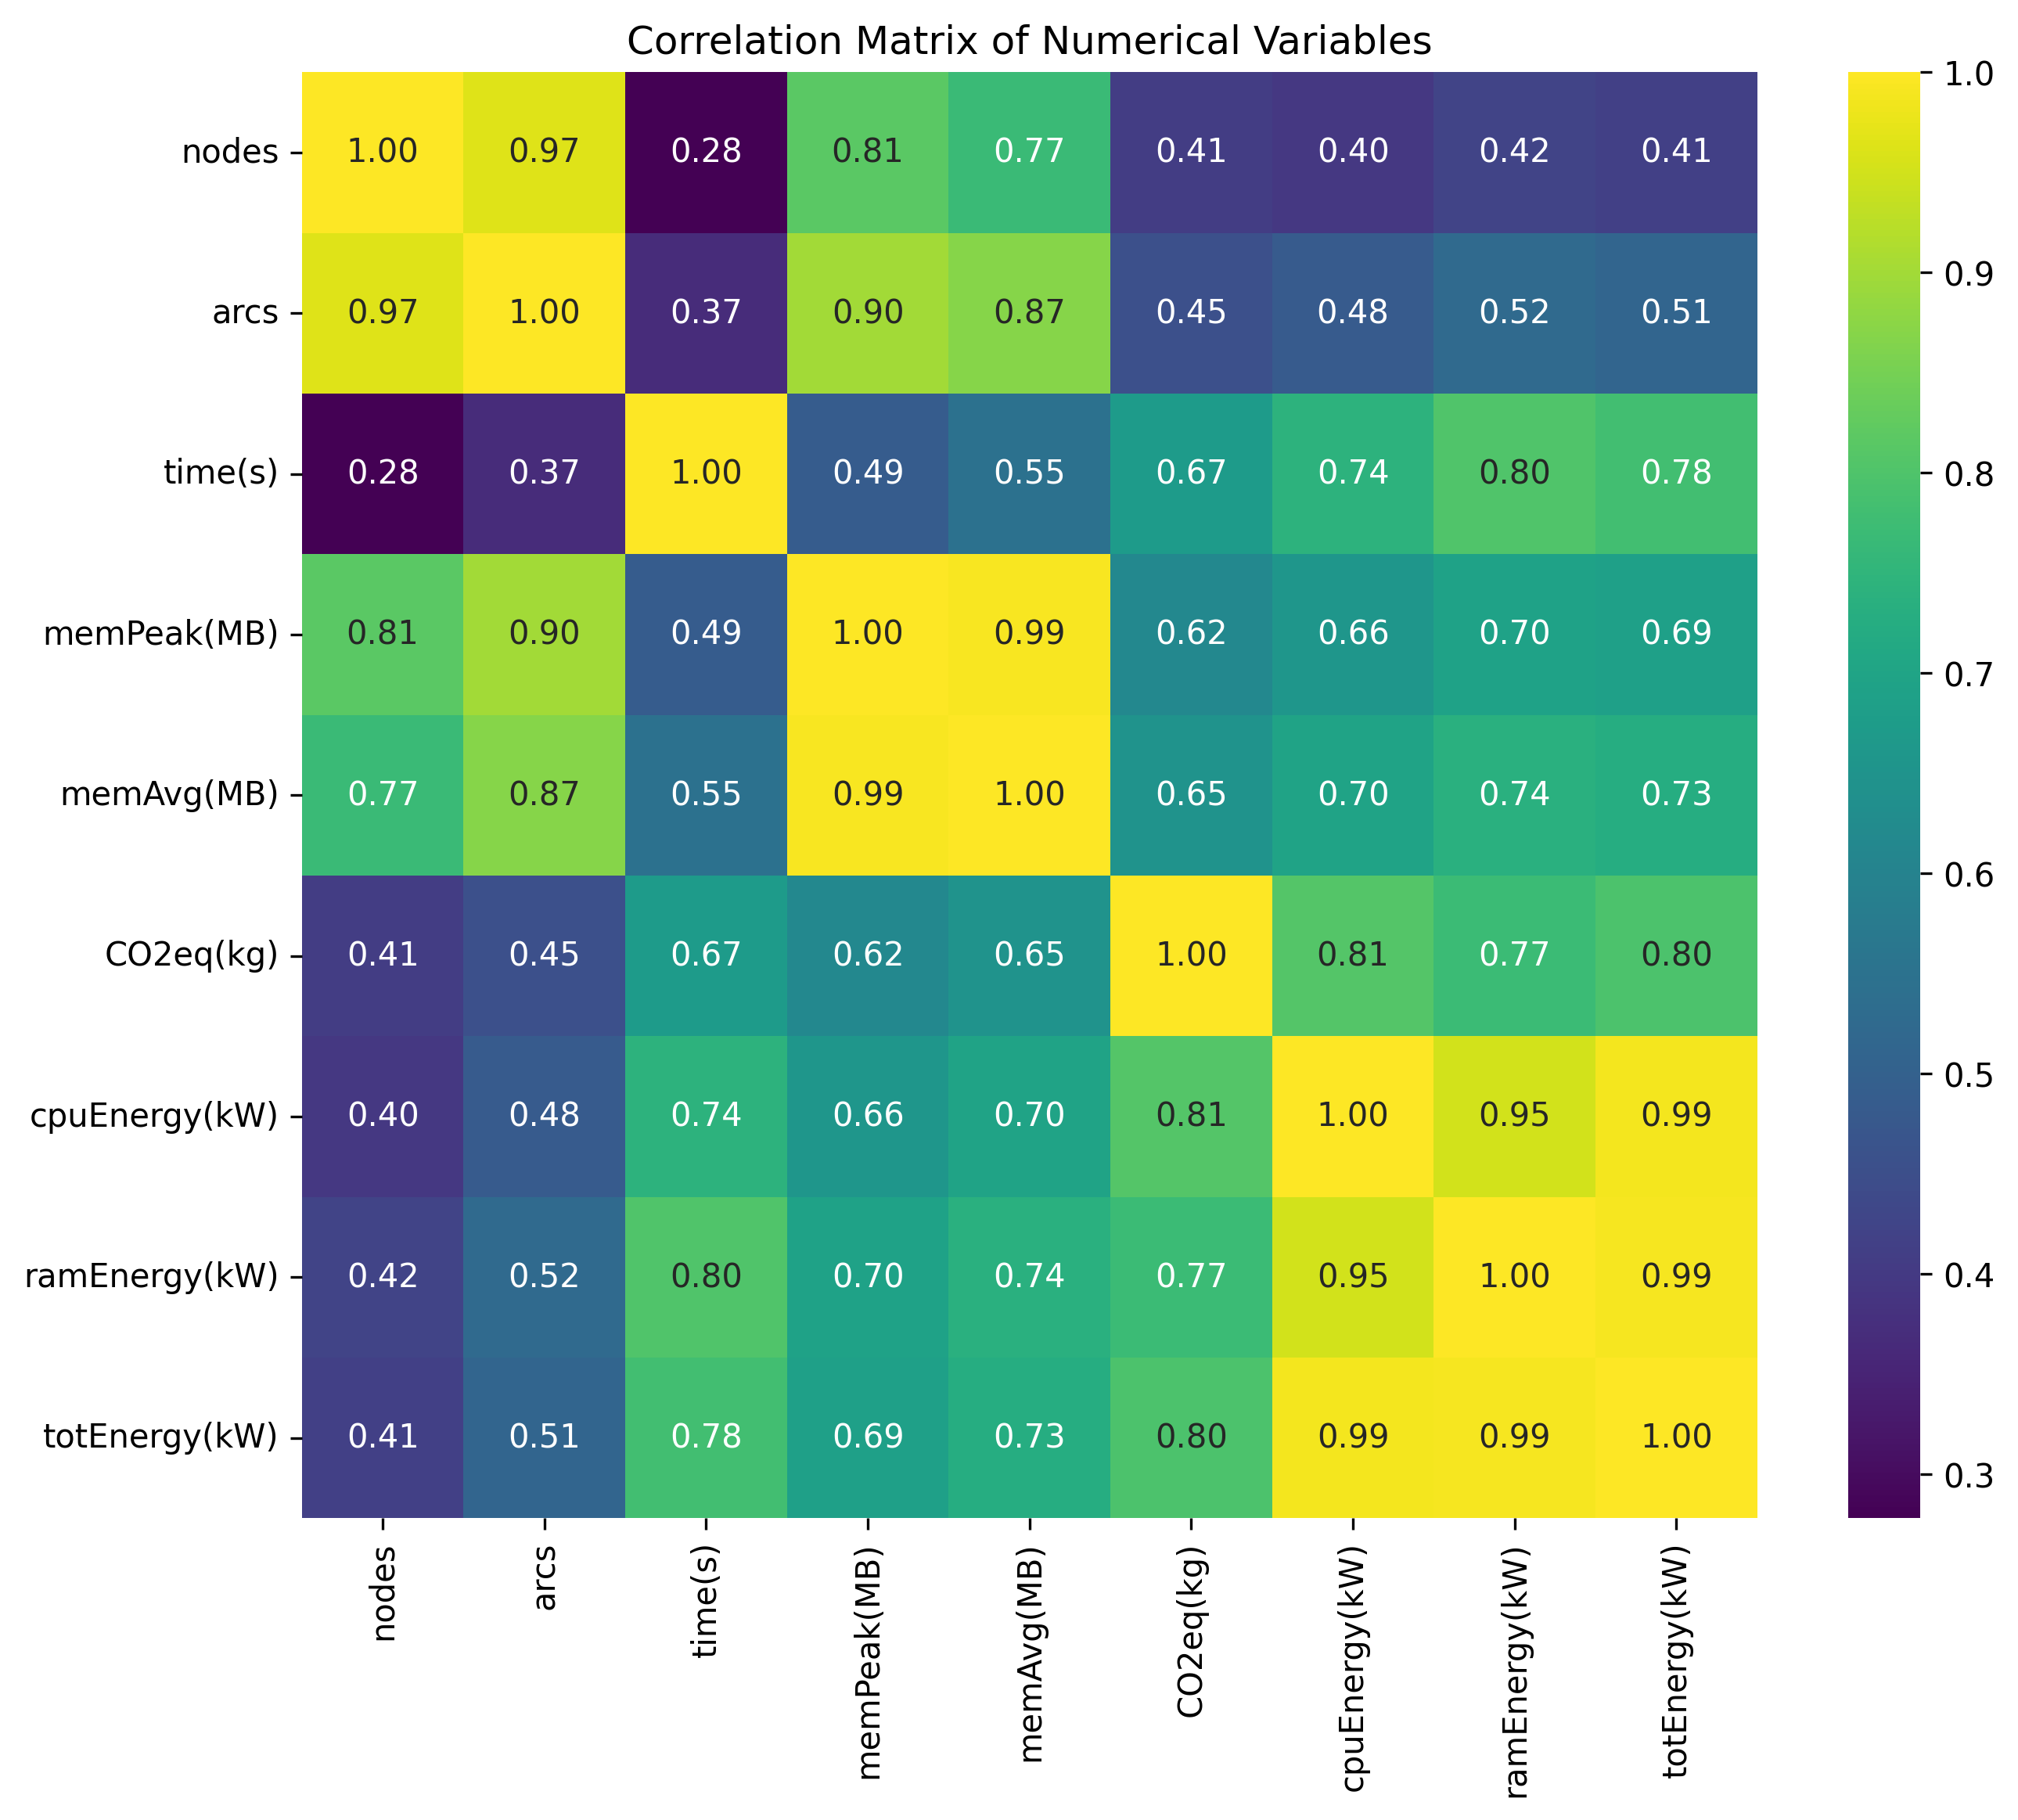
\includegraphics[width=0.8\textwidth]{imgs/max_flow_corr_mat.png}
    \caption{Correlation matrix for Min-Cut/Max-Flow Algorithms BK, EIBFS and HPF}
    \label{fig:max_flow_corr_mat}
\end{figure}

\chapter{HADA-as-a-Service}

\section{HADA Web Application}
Benchmark data was integrated into the HADA web application, requiring:
\begin{itemize}
\item Creation of JSON configuration files for each algorithm-hardware combination.
\item Specification of hyperparameters and performance targets.
\end{itemize}

Example JSON structure:
\begin{verbatim}
{
"name": "anticipate",
"HW_ID": "macbook",
"hyperparams": [
{"ID": "num_scenarios", "type": "int", "LB": 1, "UB": 100}
],
"targets": [
{"ID": "time", "LB": null, "UB": null},
{"ID": "memory", "LB": null, "UB": null},
{"ID": "emissions", "LB": null, "UB": null}
]
}
\end{verbatim}

\chapter{Conclusions}

This work extends HADA by integrating carbon emission constraints, enhancing its applicability 
for sustainable AI hardware selection. Through experimental benchmarks on laptops and HPC systems, 
we validated the framework’s ability to balance performance and environmental impact. The web-based prototype 
enables users to make informed decisions when configuring AI workloads under sustainability constraints.

\appendix

\printbibliography[heading=bibintoc] % biblatex

\acknowledgements
I'm very grateful to the inventor of the Prolog language, without whom this thesis couldn't exist. I'd also like 
to acknowledge my advisor Prof. Mario Rossi by tail-recursively acknowledging my advisor.
	
\end{document}